%\documentclass{article}
%\usepackage[utf8]{inputenc}

\documentclass[12pt]{article}
\usepackage{graphicx} % This lets you include figures
\usepackage{hyperref} % This lets you make links to web locations
\graphicspath{ {./images/} }

\usepackage[rightcaption]{sidecap}
\usepackage{caption}
\usepackage{subcaption}
\usepackage{hyperref}

\usepackage{float}

\usepackage{imakeidx}

\makeindex


\title{Manual}
\author{Beau De Clercq}
\date{July 2019}

\begin{document}
\maketitle{}

\tableofcontents

\clearpage
\newpage

\section{Setting Up for the first time}
\subsection{Docker}
In order for this interface to work, a working version of Docker needs to be installed and running on your machine.\\
For this, please follow the steps found at \url{https://docs.docker.com/get-started/}.\\
Linux users will need to run the \texttt{install.sh} script to ensure a correct working.

\subsection{Creating the databases}
Once Docker is up and running it is time to make everything ready for use.\\
The first thing you need to do is execute the \texttt{run.sh} script on Mac/Linux while Windows users will need to execute the \texttt{run.bat} script.\\
When the services are up and running the user will need to open a second terminal and execute the \texttt{create\_dbs.sh} script on Mac/Linux or the \texttt{create\_dbs.bat} script on Windows. This  will create the necessary tables and also fill the database with all stops available at that time in order to prevent long loading times when using the app.
\newpage

\section{Usage}
After completing the set-up, the app can be launched by running \texttt{run} script for the corresponding OS and will be available at \url{http://localhost:5000/}.\\
Following pages will describe how the different aspects can be used.
\newpage
\subsection{Home}
\begin{center}
	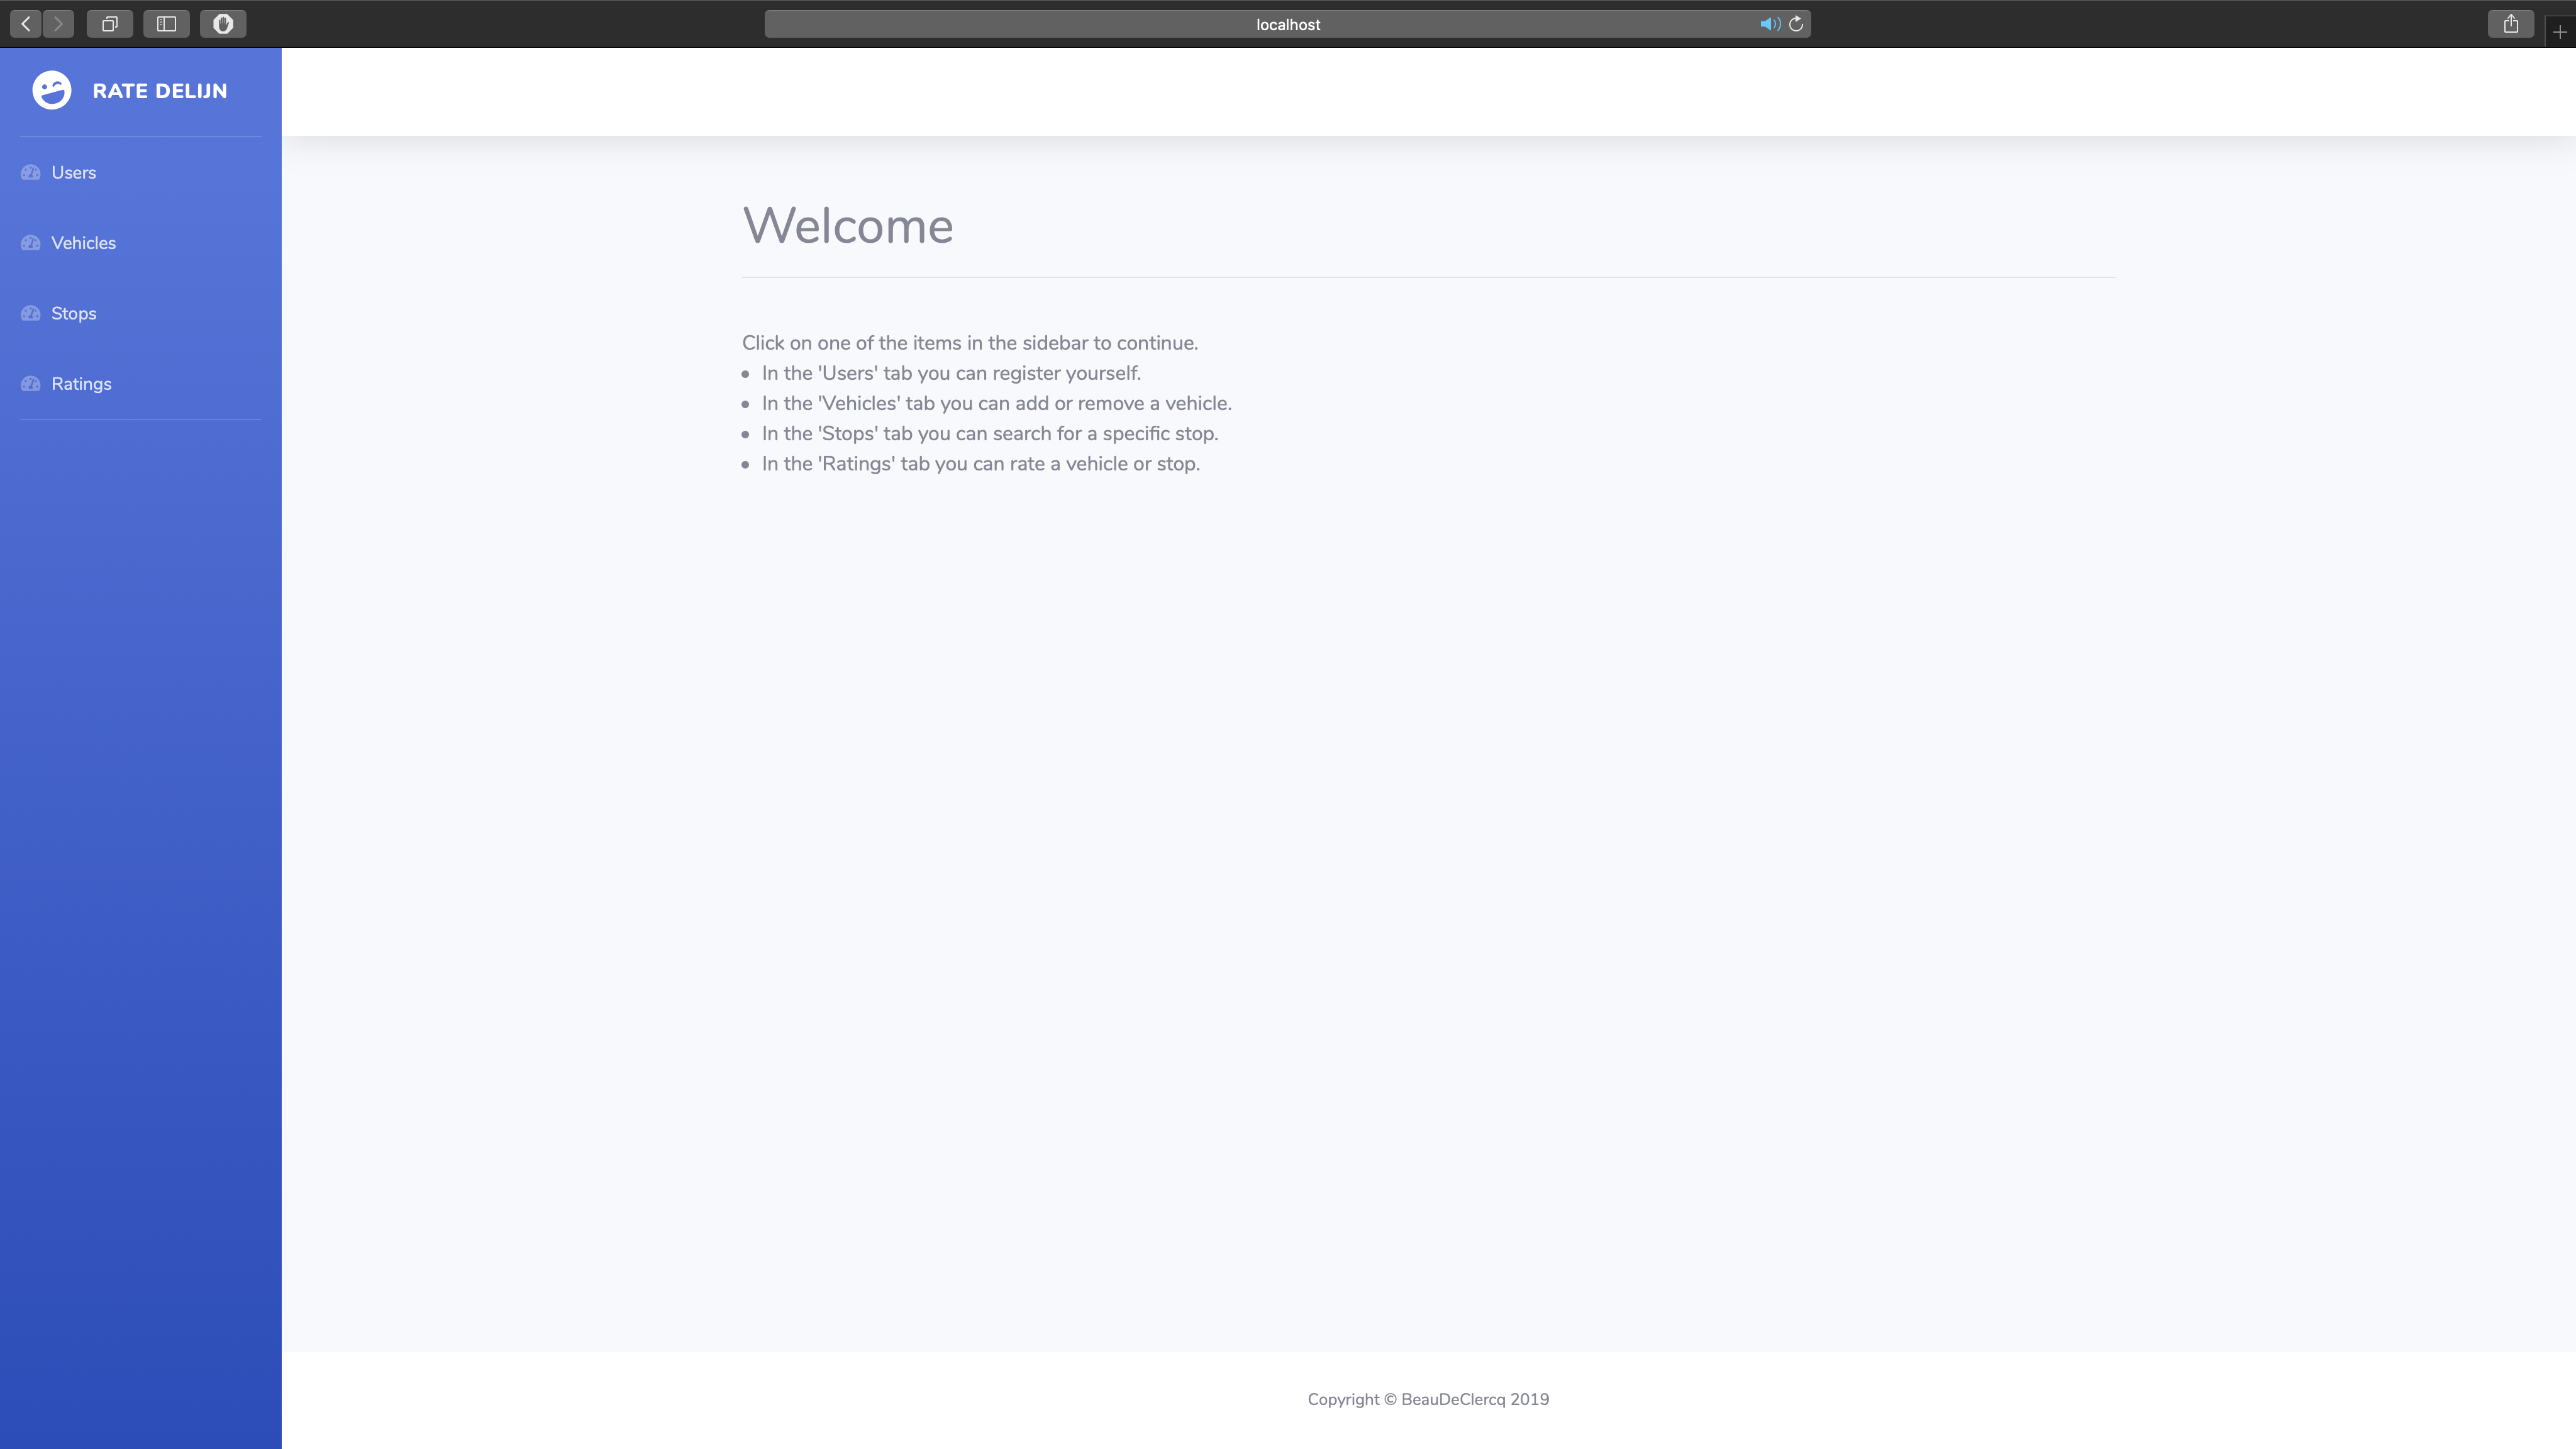
\includegraphics[width=\linewidth]{Images/Home_screen.png}
	\captionof{figure}{Home screen}
\end{center}
The home page of the app provides a small description of what can be done in any of the individual tabs.

\subsection{Users tab}
\begin{center}
	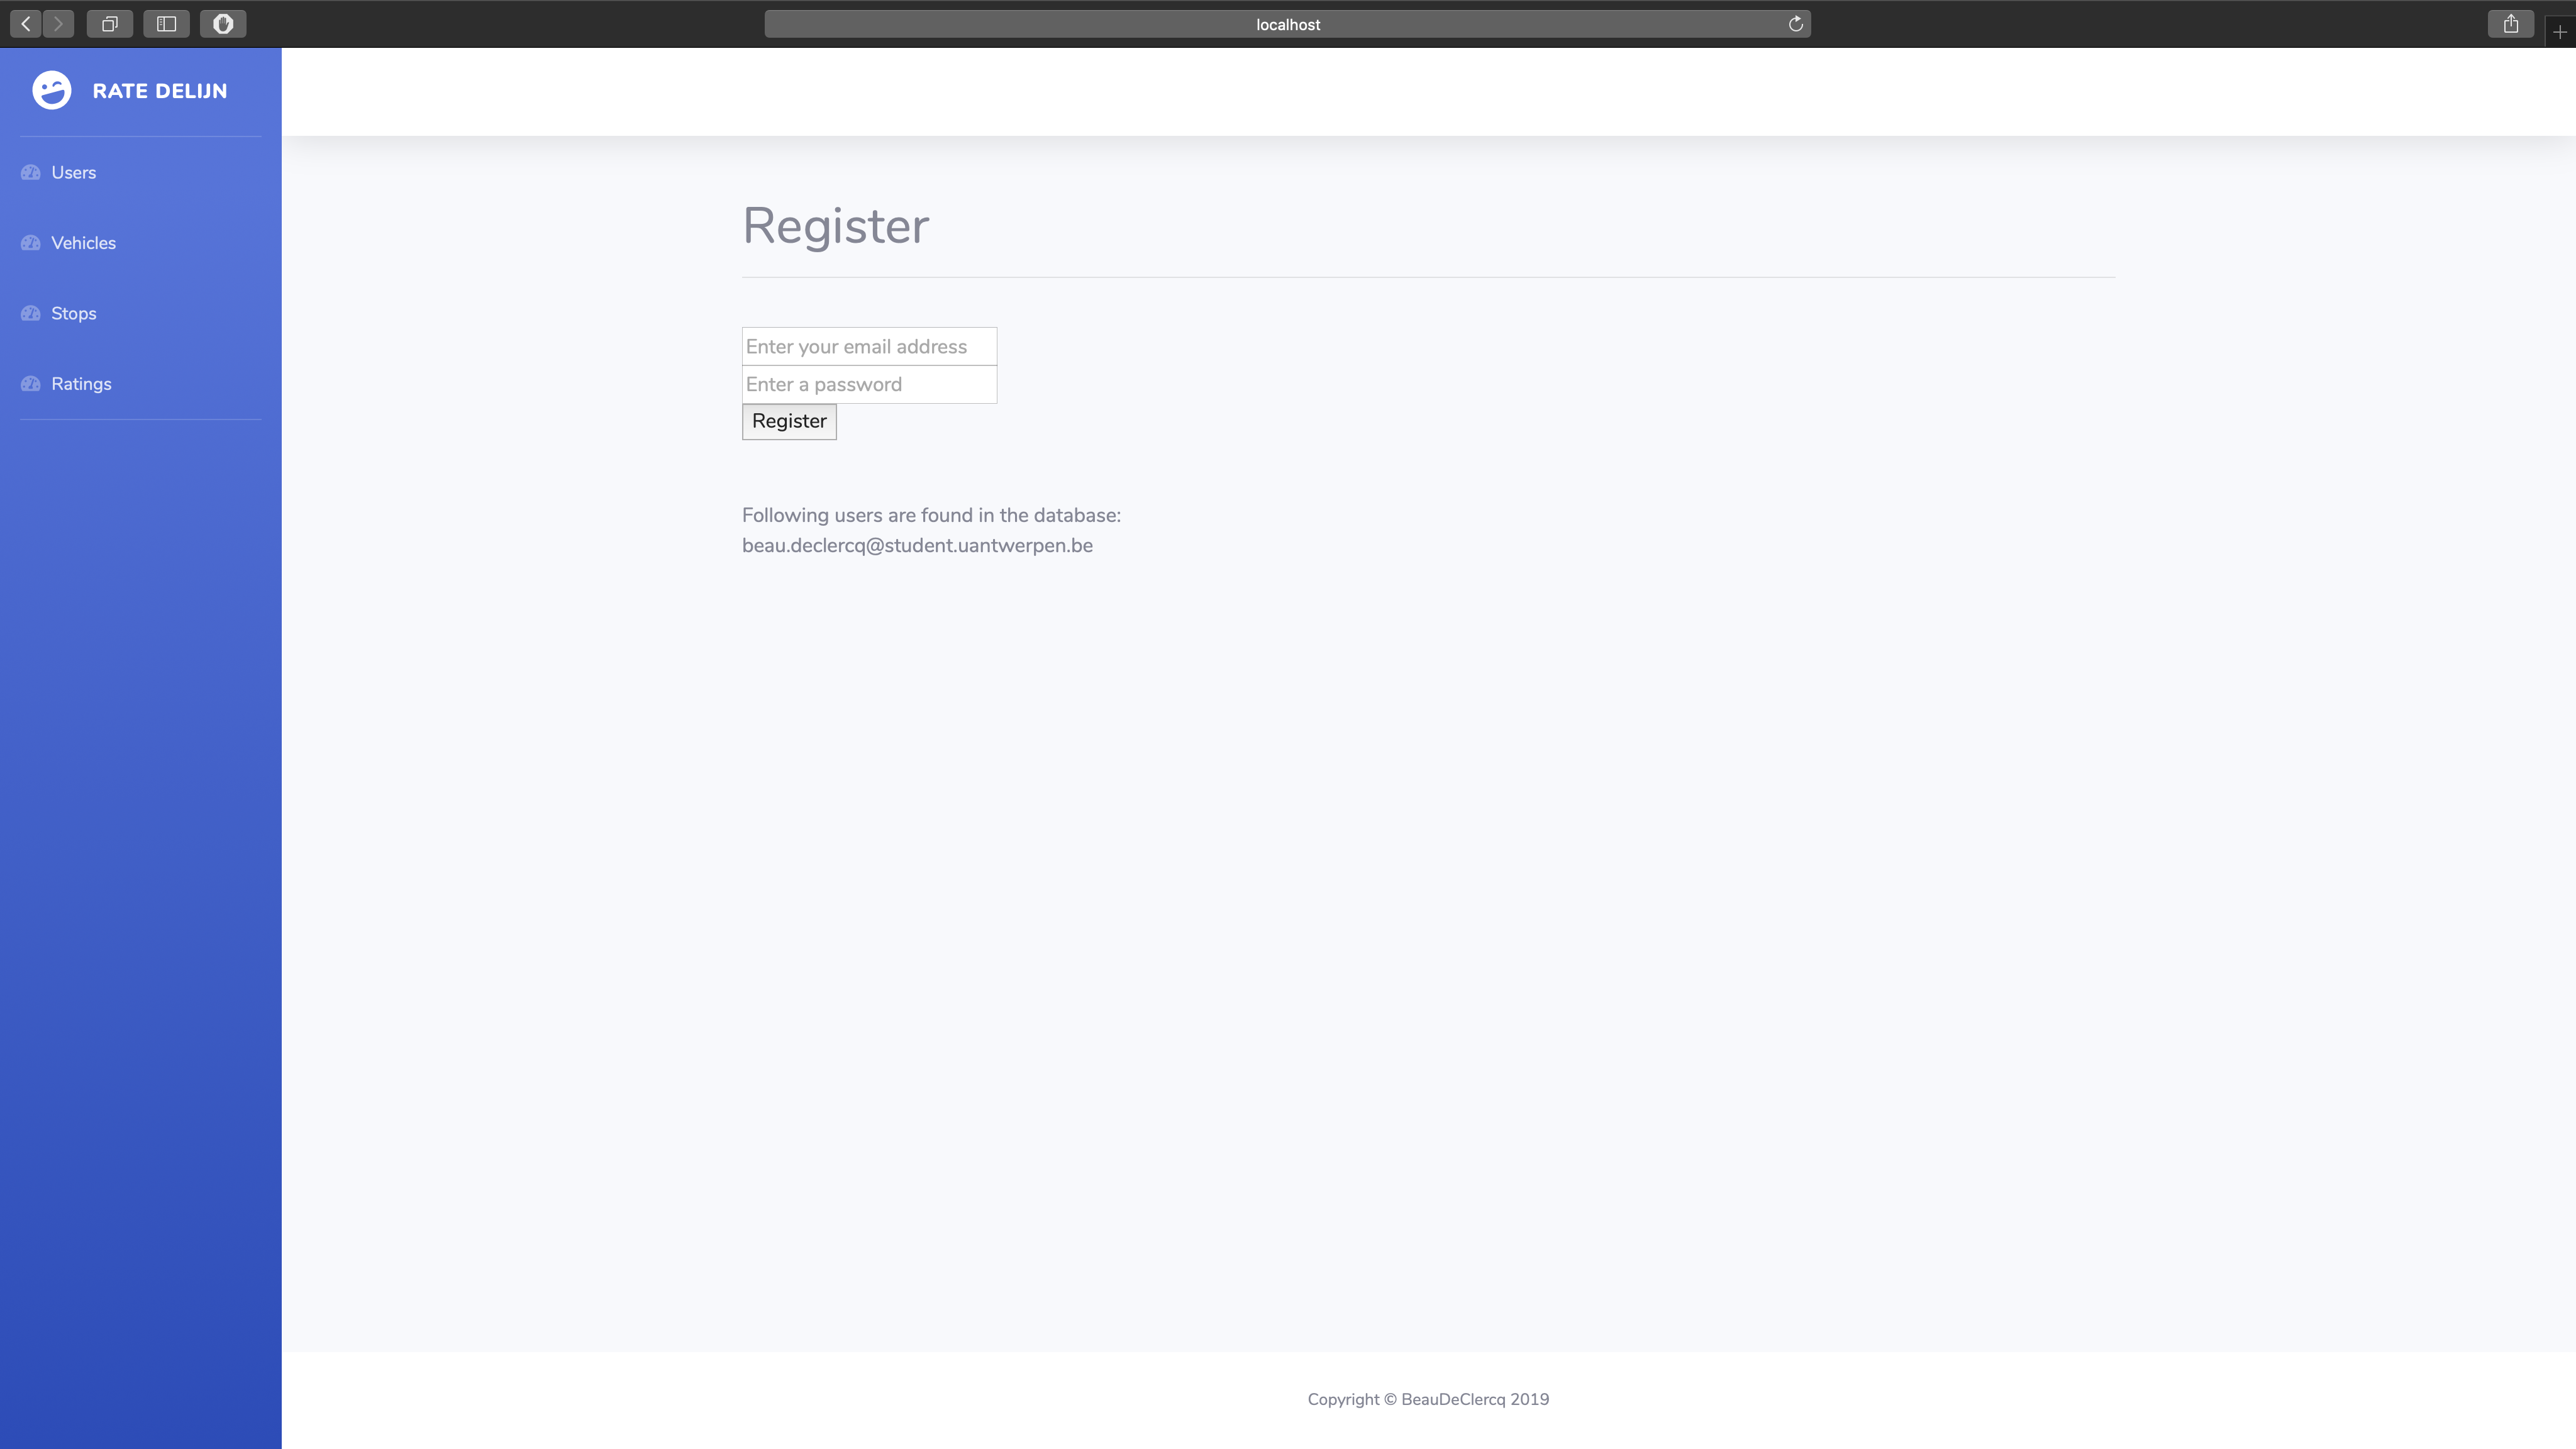
\includegraphics[width=\linewidth]{Images/Users_tab.png}
	\captionof{figure}{Users tab}
\end{center}
In the \textbf{Users} tab, users can register themselves by filling in their email address and a password they want to use throughout the system.\\
After submitting the form, the user will be taken back to the home page where a message will be shown telling whether the registration has succeeded or not.\\
Under the registration form the user can view a list of all registered email addresses in the system. This may prevent users from unintentionally registering themselves multiple times.

\subsection{Vehicles tab}
\begin{center}
	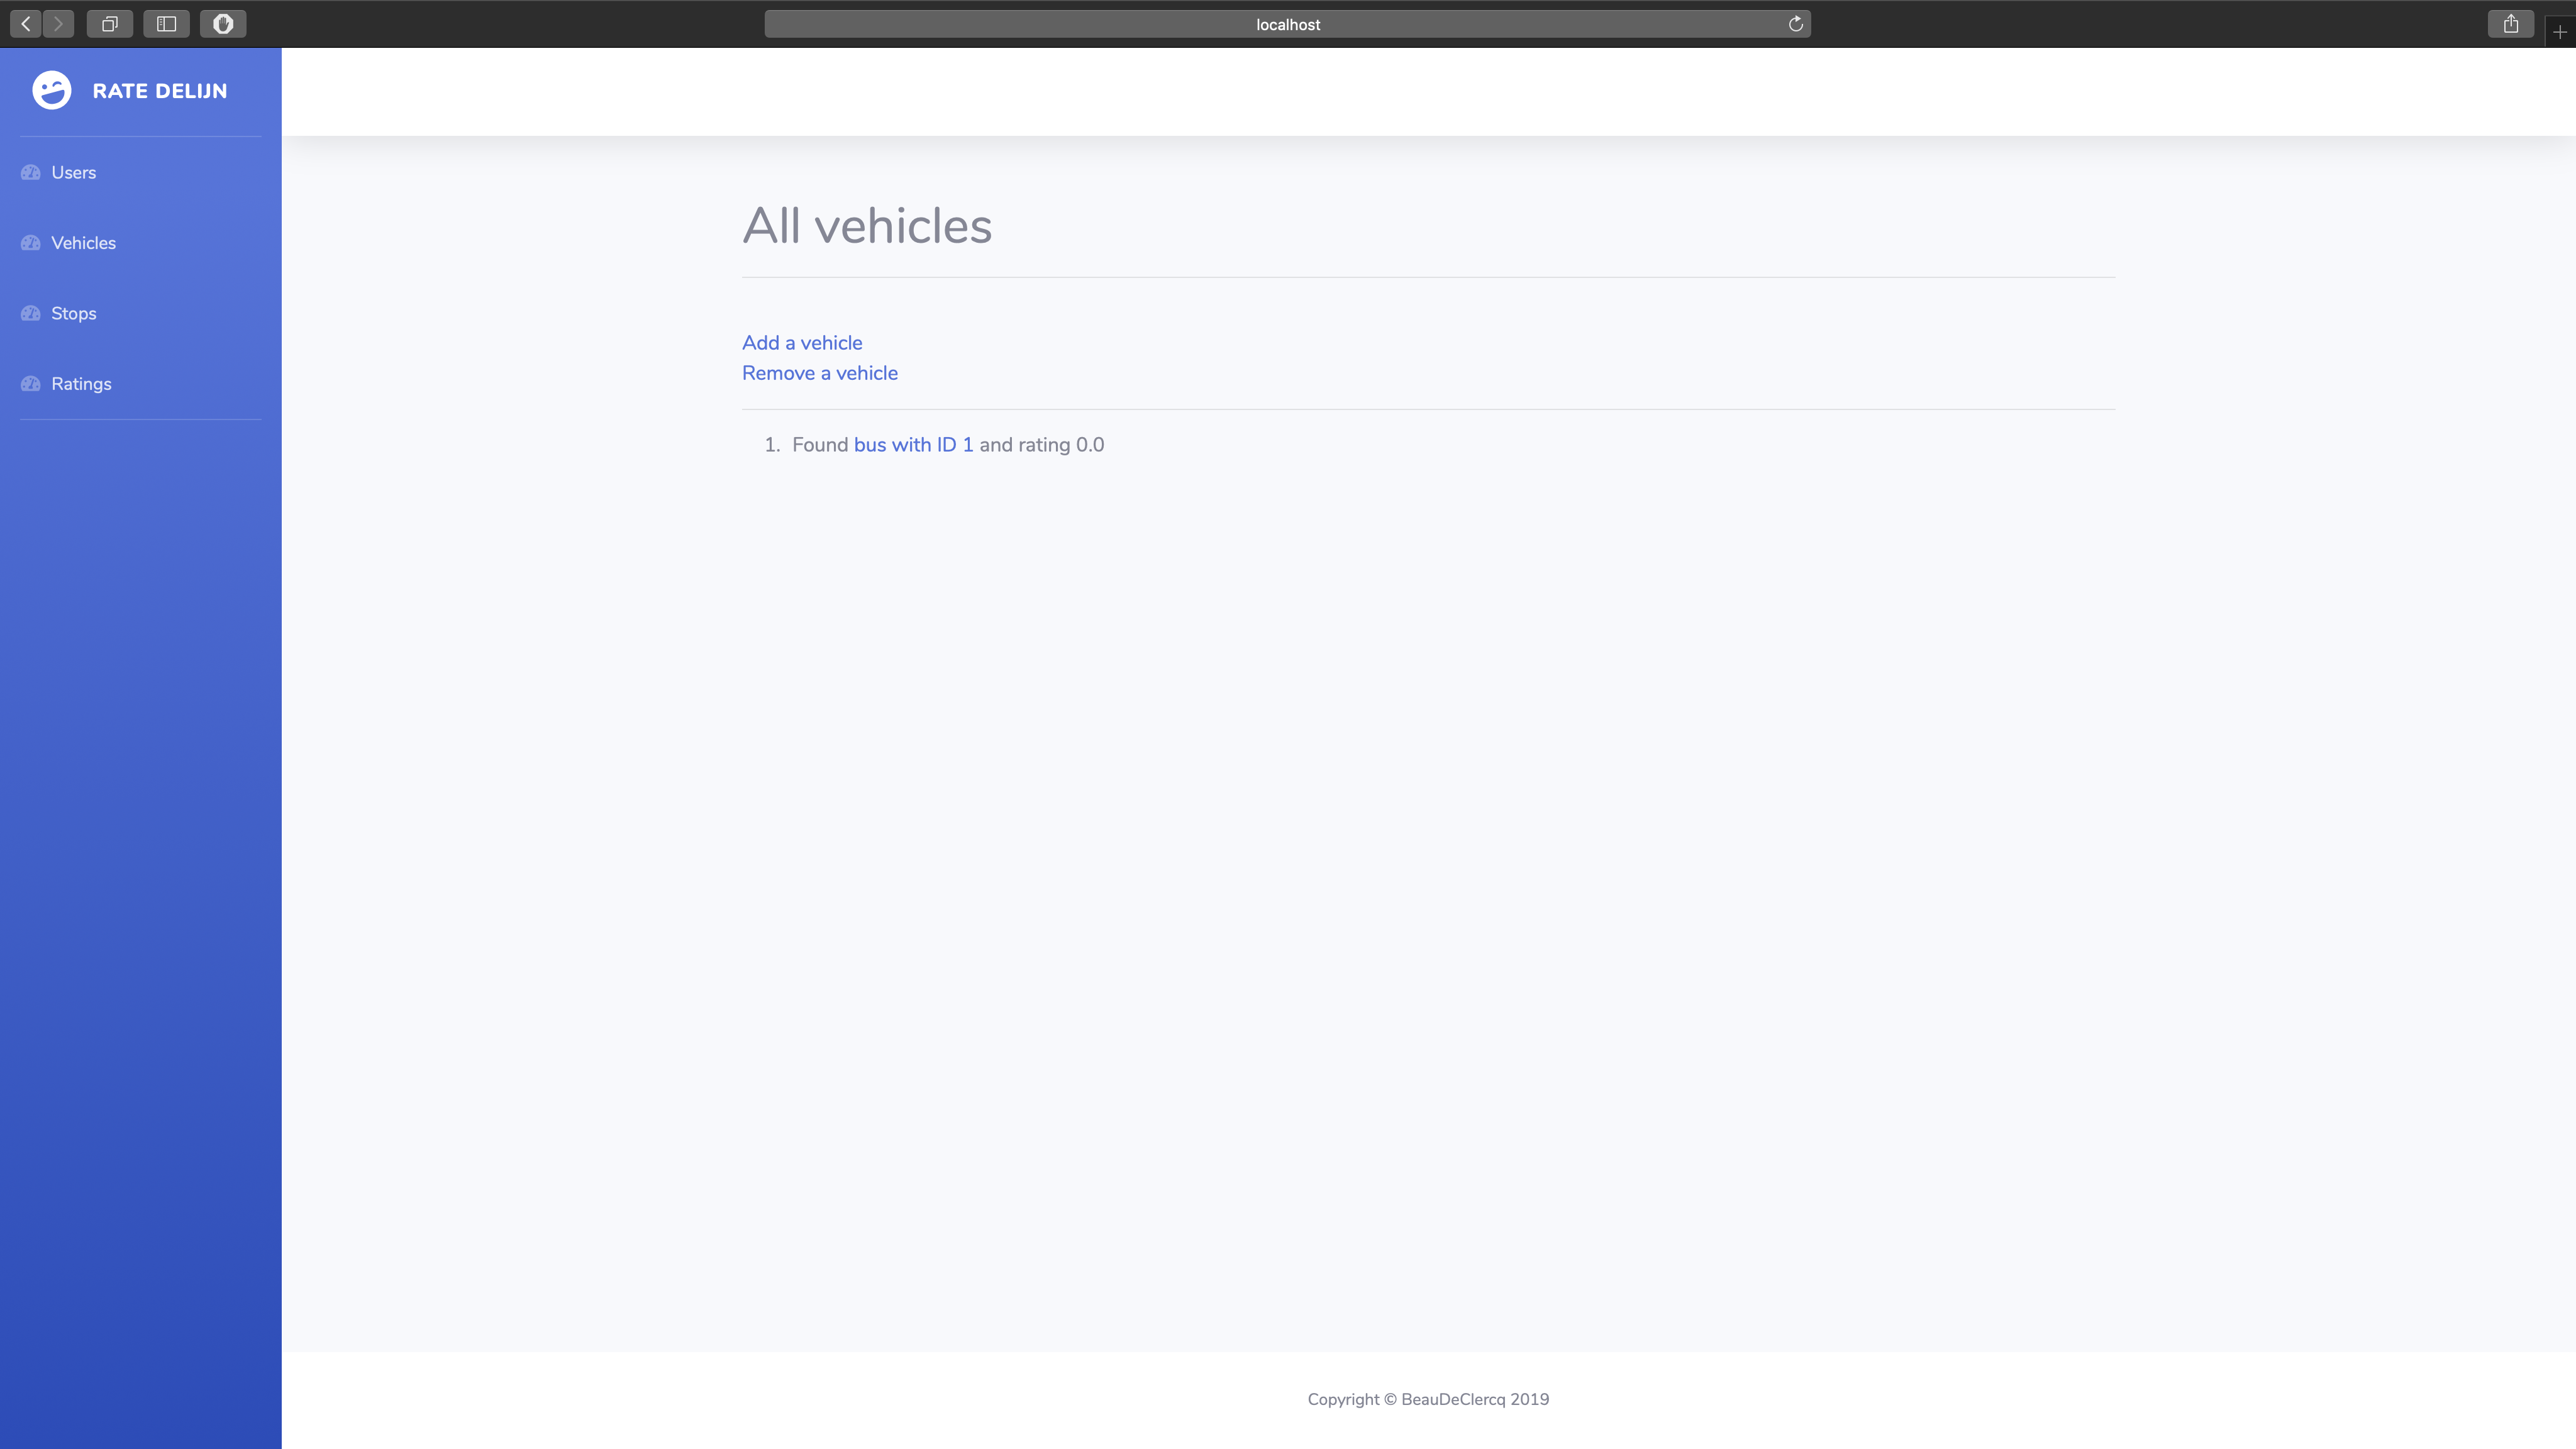
\includegraphics[width=\linewidth]{Images/Vehicles_tab.png}
	\captionof{figure}{Vehicles tab}
\end{center}
In the \textbf{Vehicles} tab, registered users can add a new vehicle or remove an existing vehicle.\\
In this tab, registered and unregistered users alike can also see a list of all vehicles currently registered. By clicking on any vehicle the user will be taken to a page that will provide more details.

\subsubsection{Adding a vehicle}
\begin{center}
	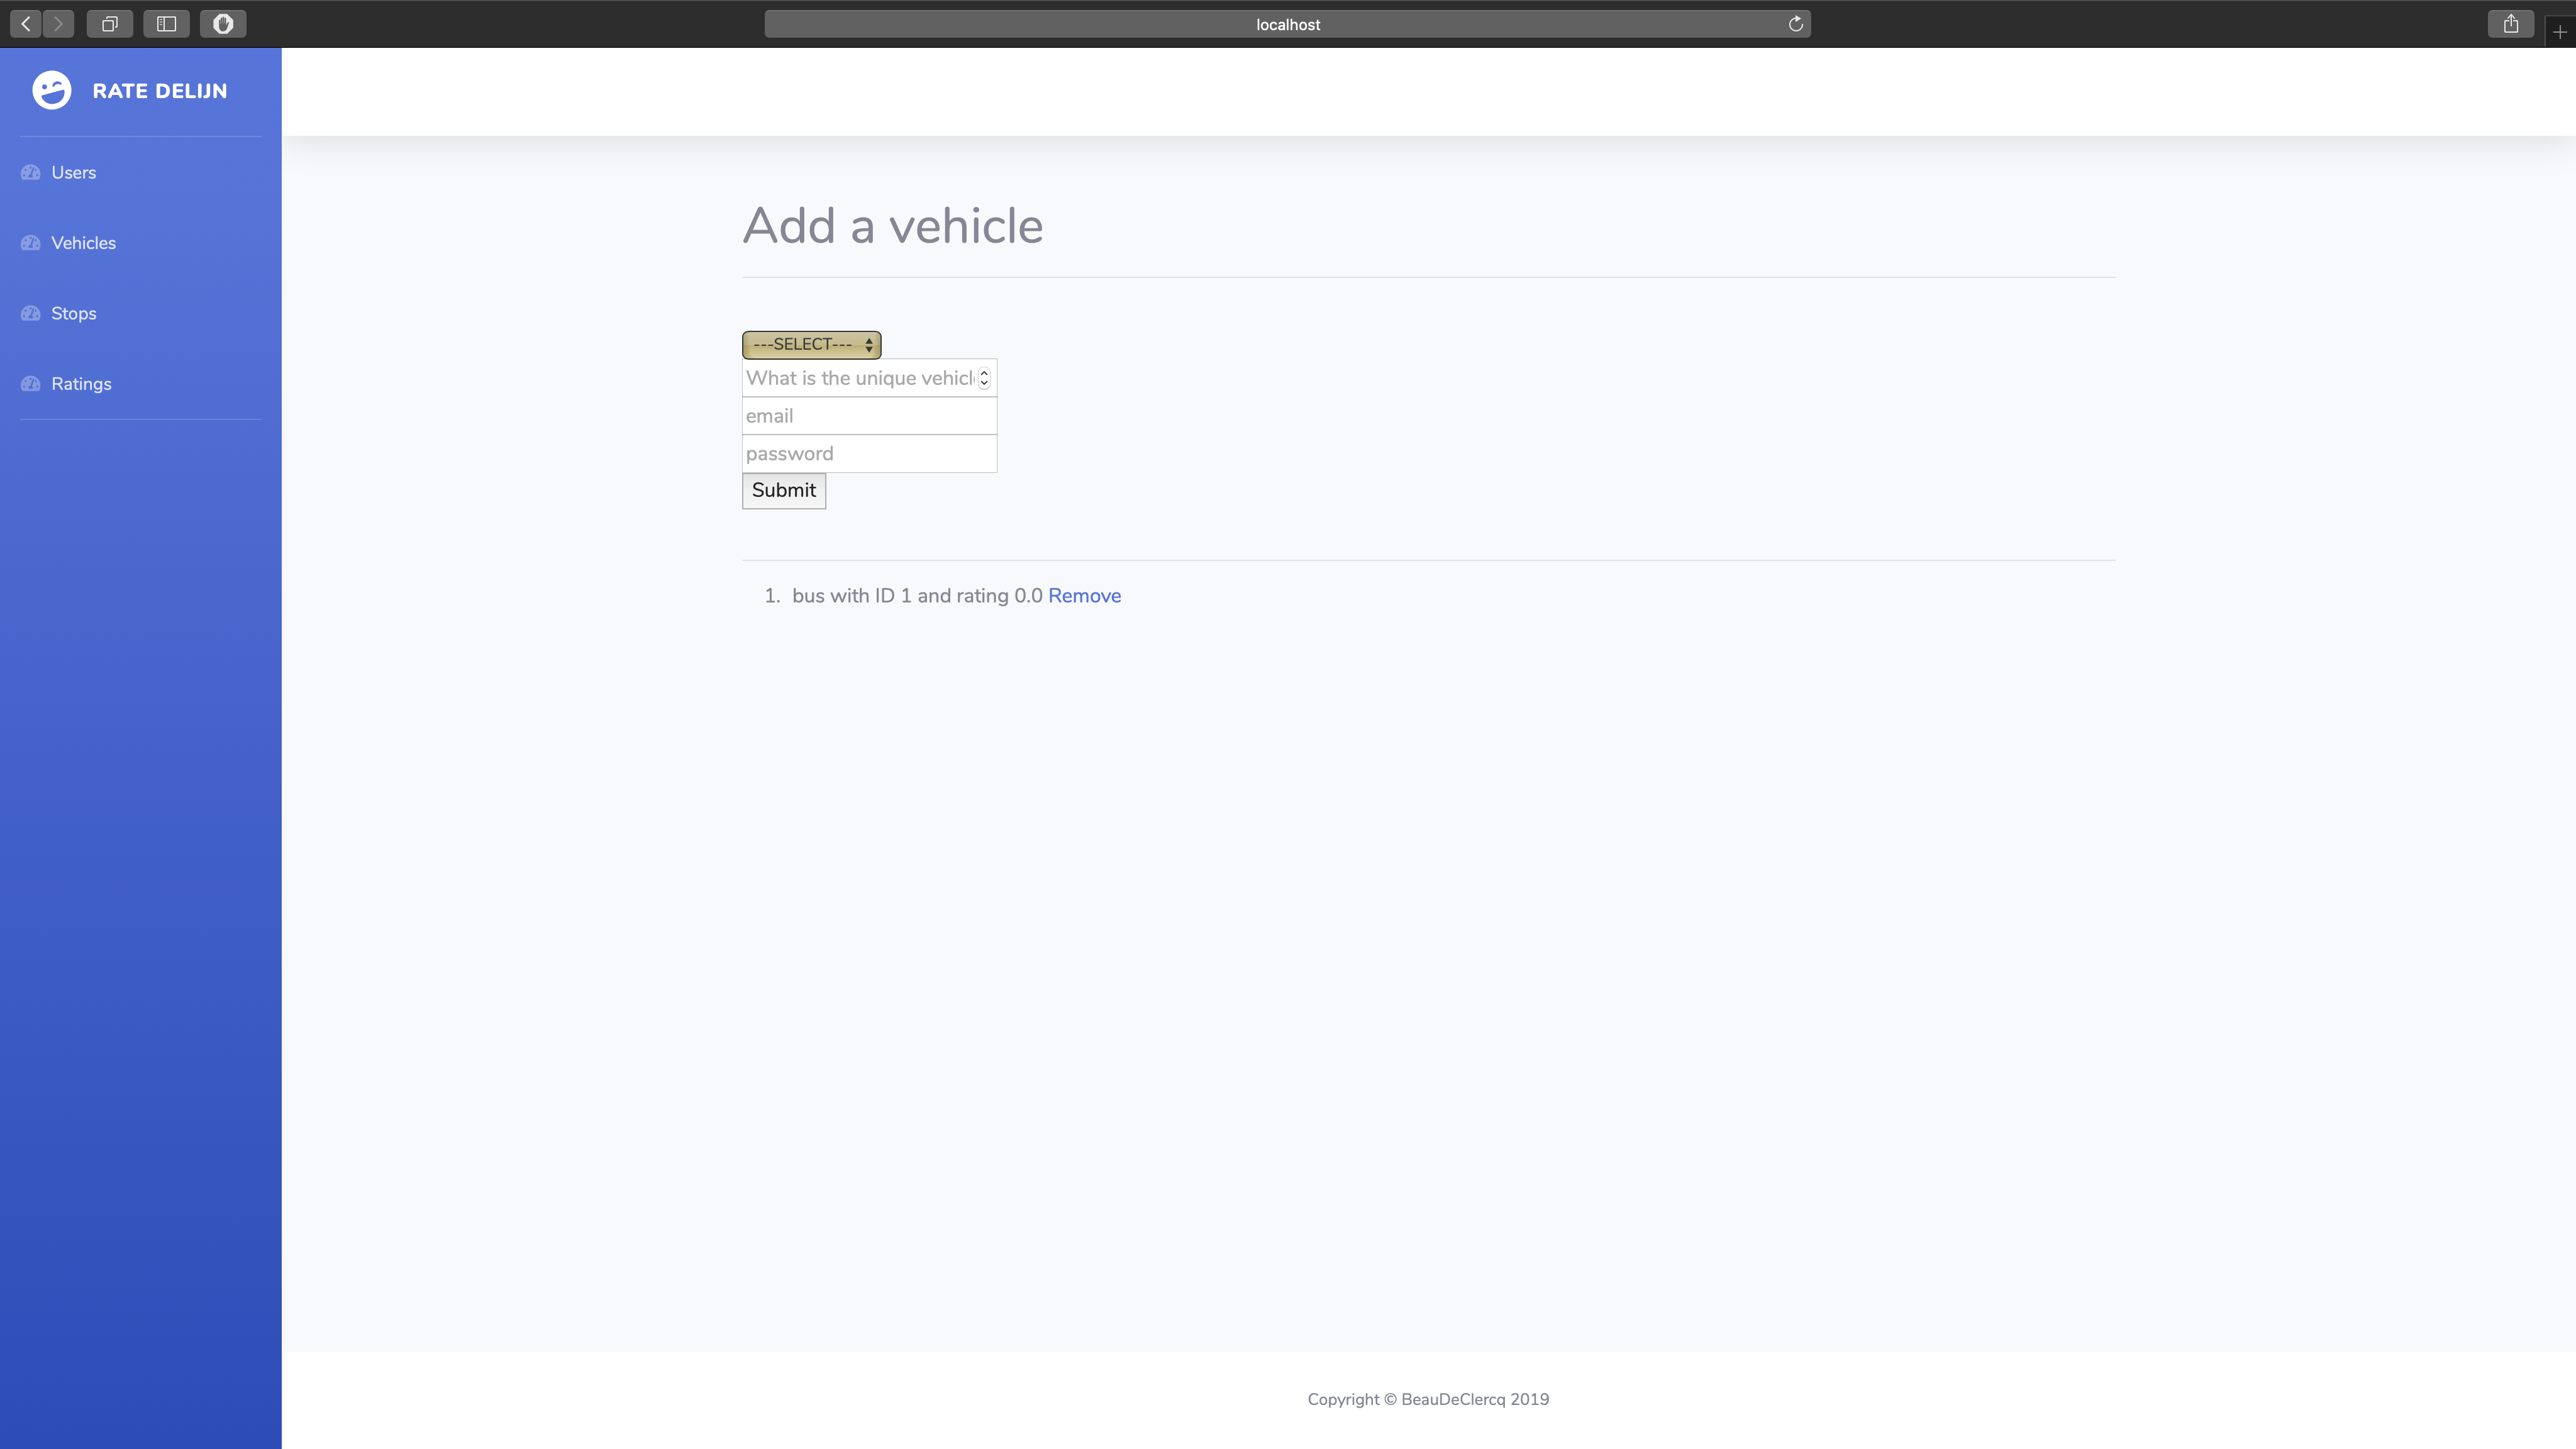
\includegraphics[width=\linewidth]{Images/Add_vehicle.png}
	\captionof{figure}{Adding a vehicle}
\end{center}
A user can add a vehicle to the database by filling in the required fields and authenticating. Once the form is submitted, the user will be redirected to the home page where a message will be shown telling whether the operation was successful or not.\\
Underneath the form, users can see a list of all vehicles currently registered in the system to prevent them from entering a vehicle with the same ID multiple times.\\
If a user thinks that a vehicle has been added with a wrong ID, that vehicle can be removed by clicking the `Remove' button and following the removal procedure.

\subsubsection{Removing a vehicle}
\begin{center}
	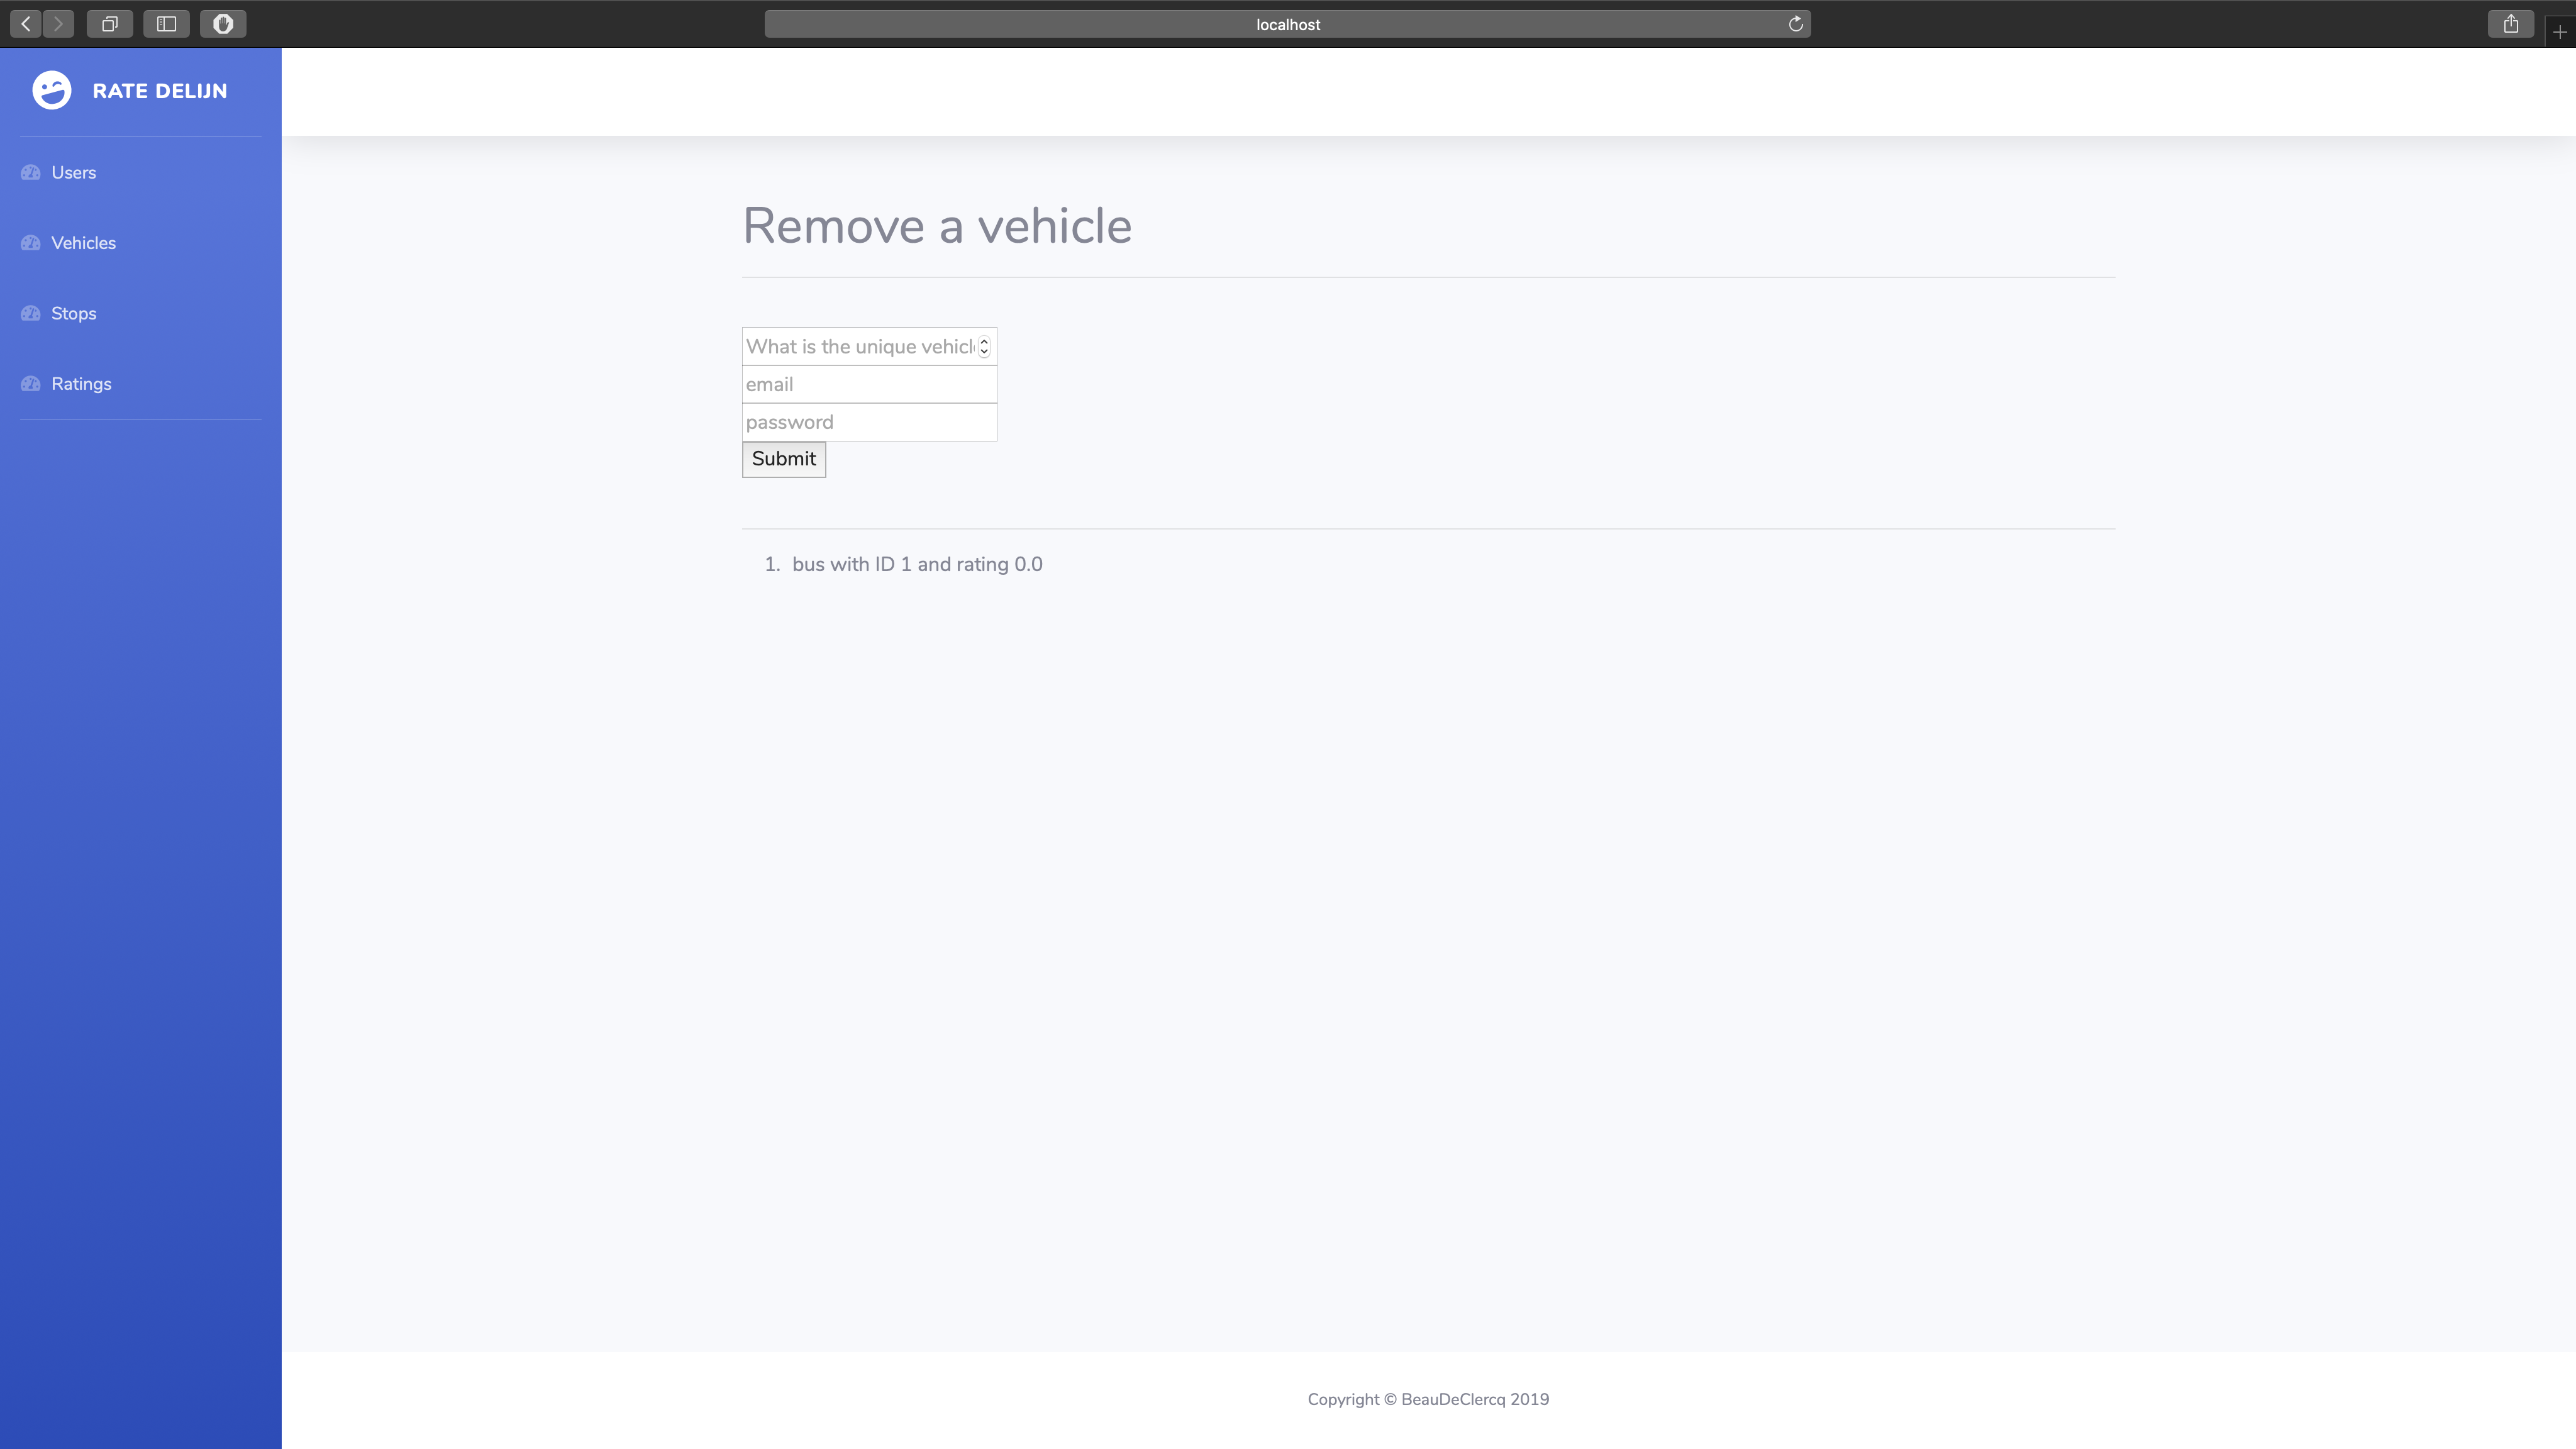
\includegraphics[width=\linewidth]{Images/Remove_vehicle.png}
	\captionof{figure}{Removing a vehicle}
\end{center}
A user can remove a vehicle from the database by filling in the required fields and authenticating. Once the form is submitted, the user will be redirected to the home page where a message will be shown telling whether the operation was successful or not.\\

\subsubsection{Vehicle details}
\begin{center}
	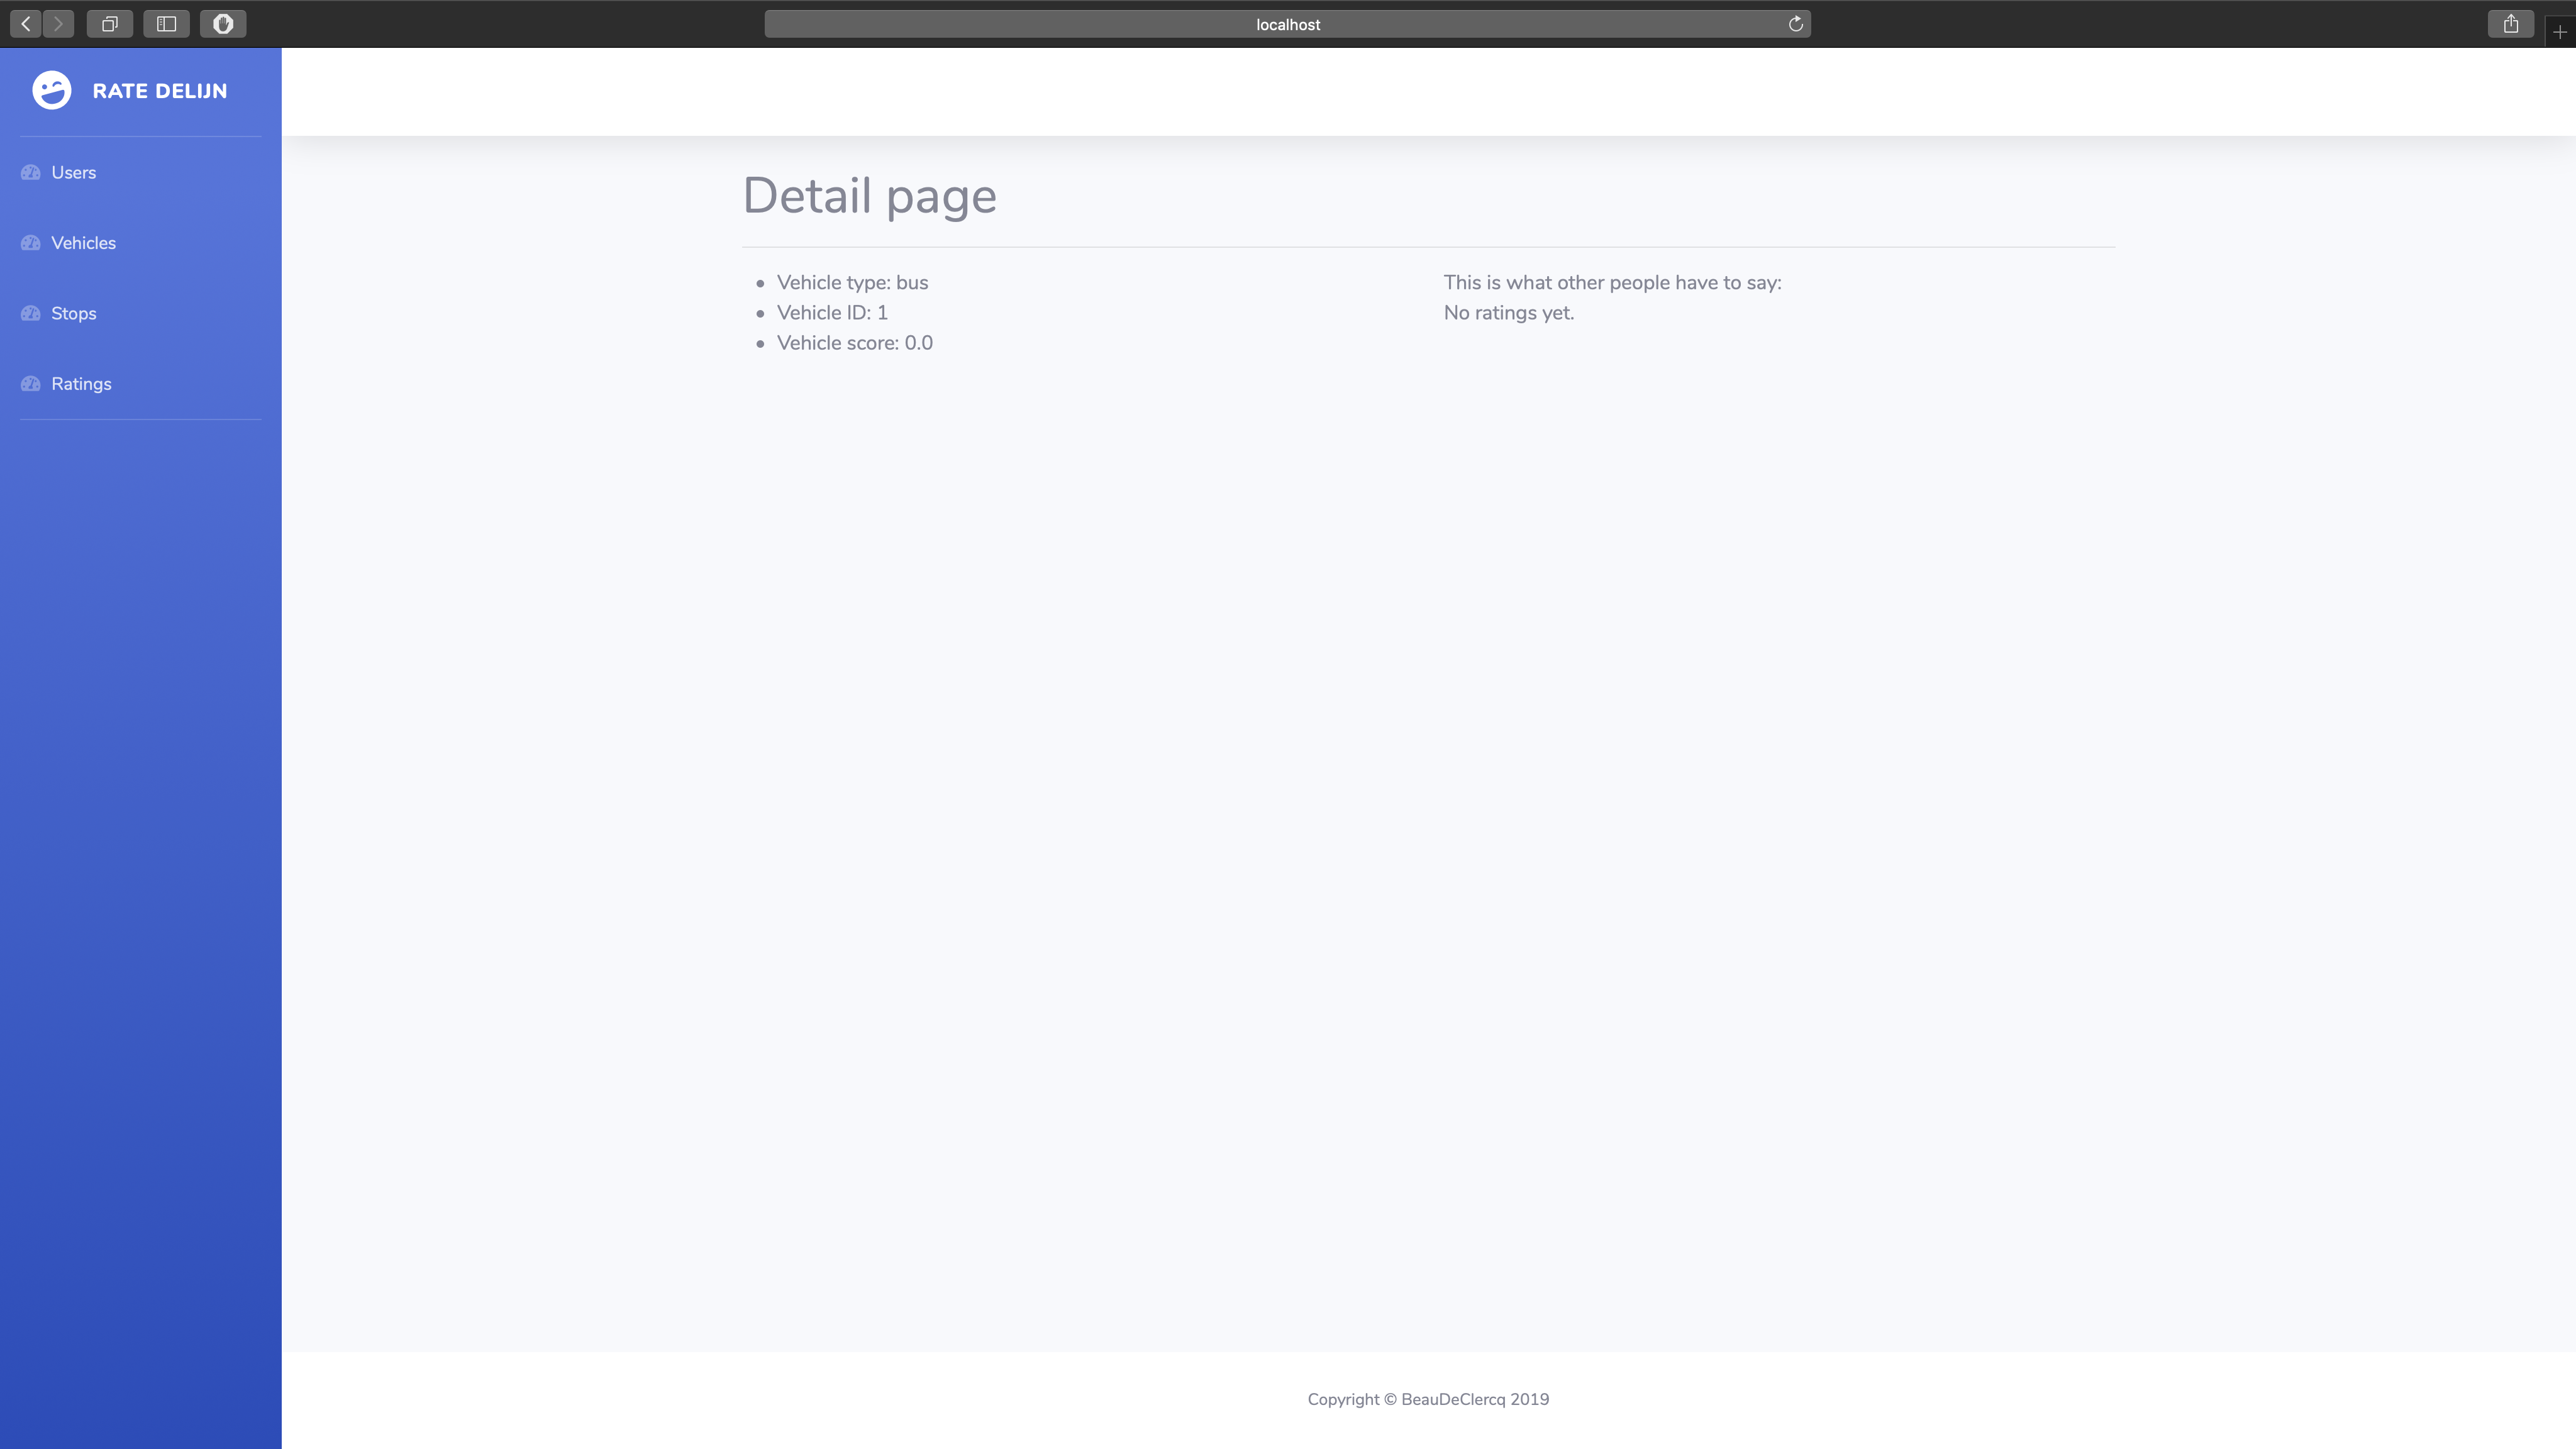
\includegraphics[width=\linewidth]{Images/Vehicle_details.png}
	\captionof{figure}{Details a vehicle}
\end{center}
On the details page, users can see the details about the vehicle and read all ratings that are currently submitted.

\subsection{Stops tab}
\begin{center}
	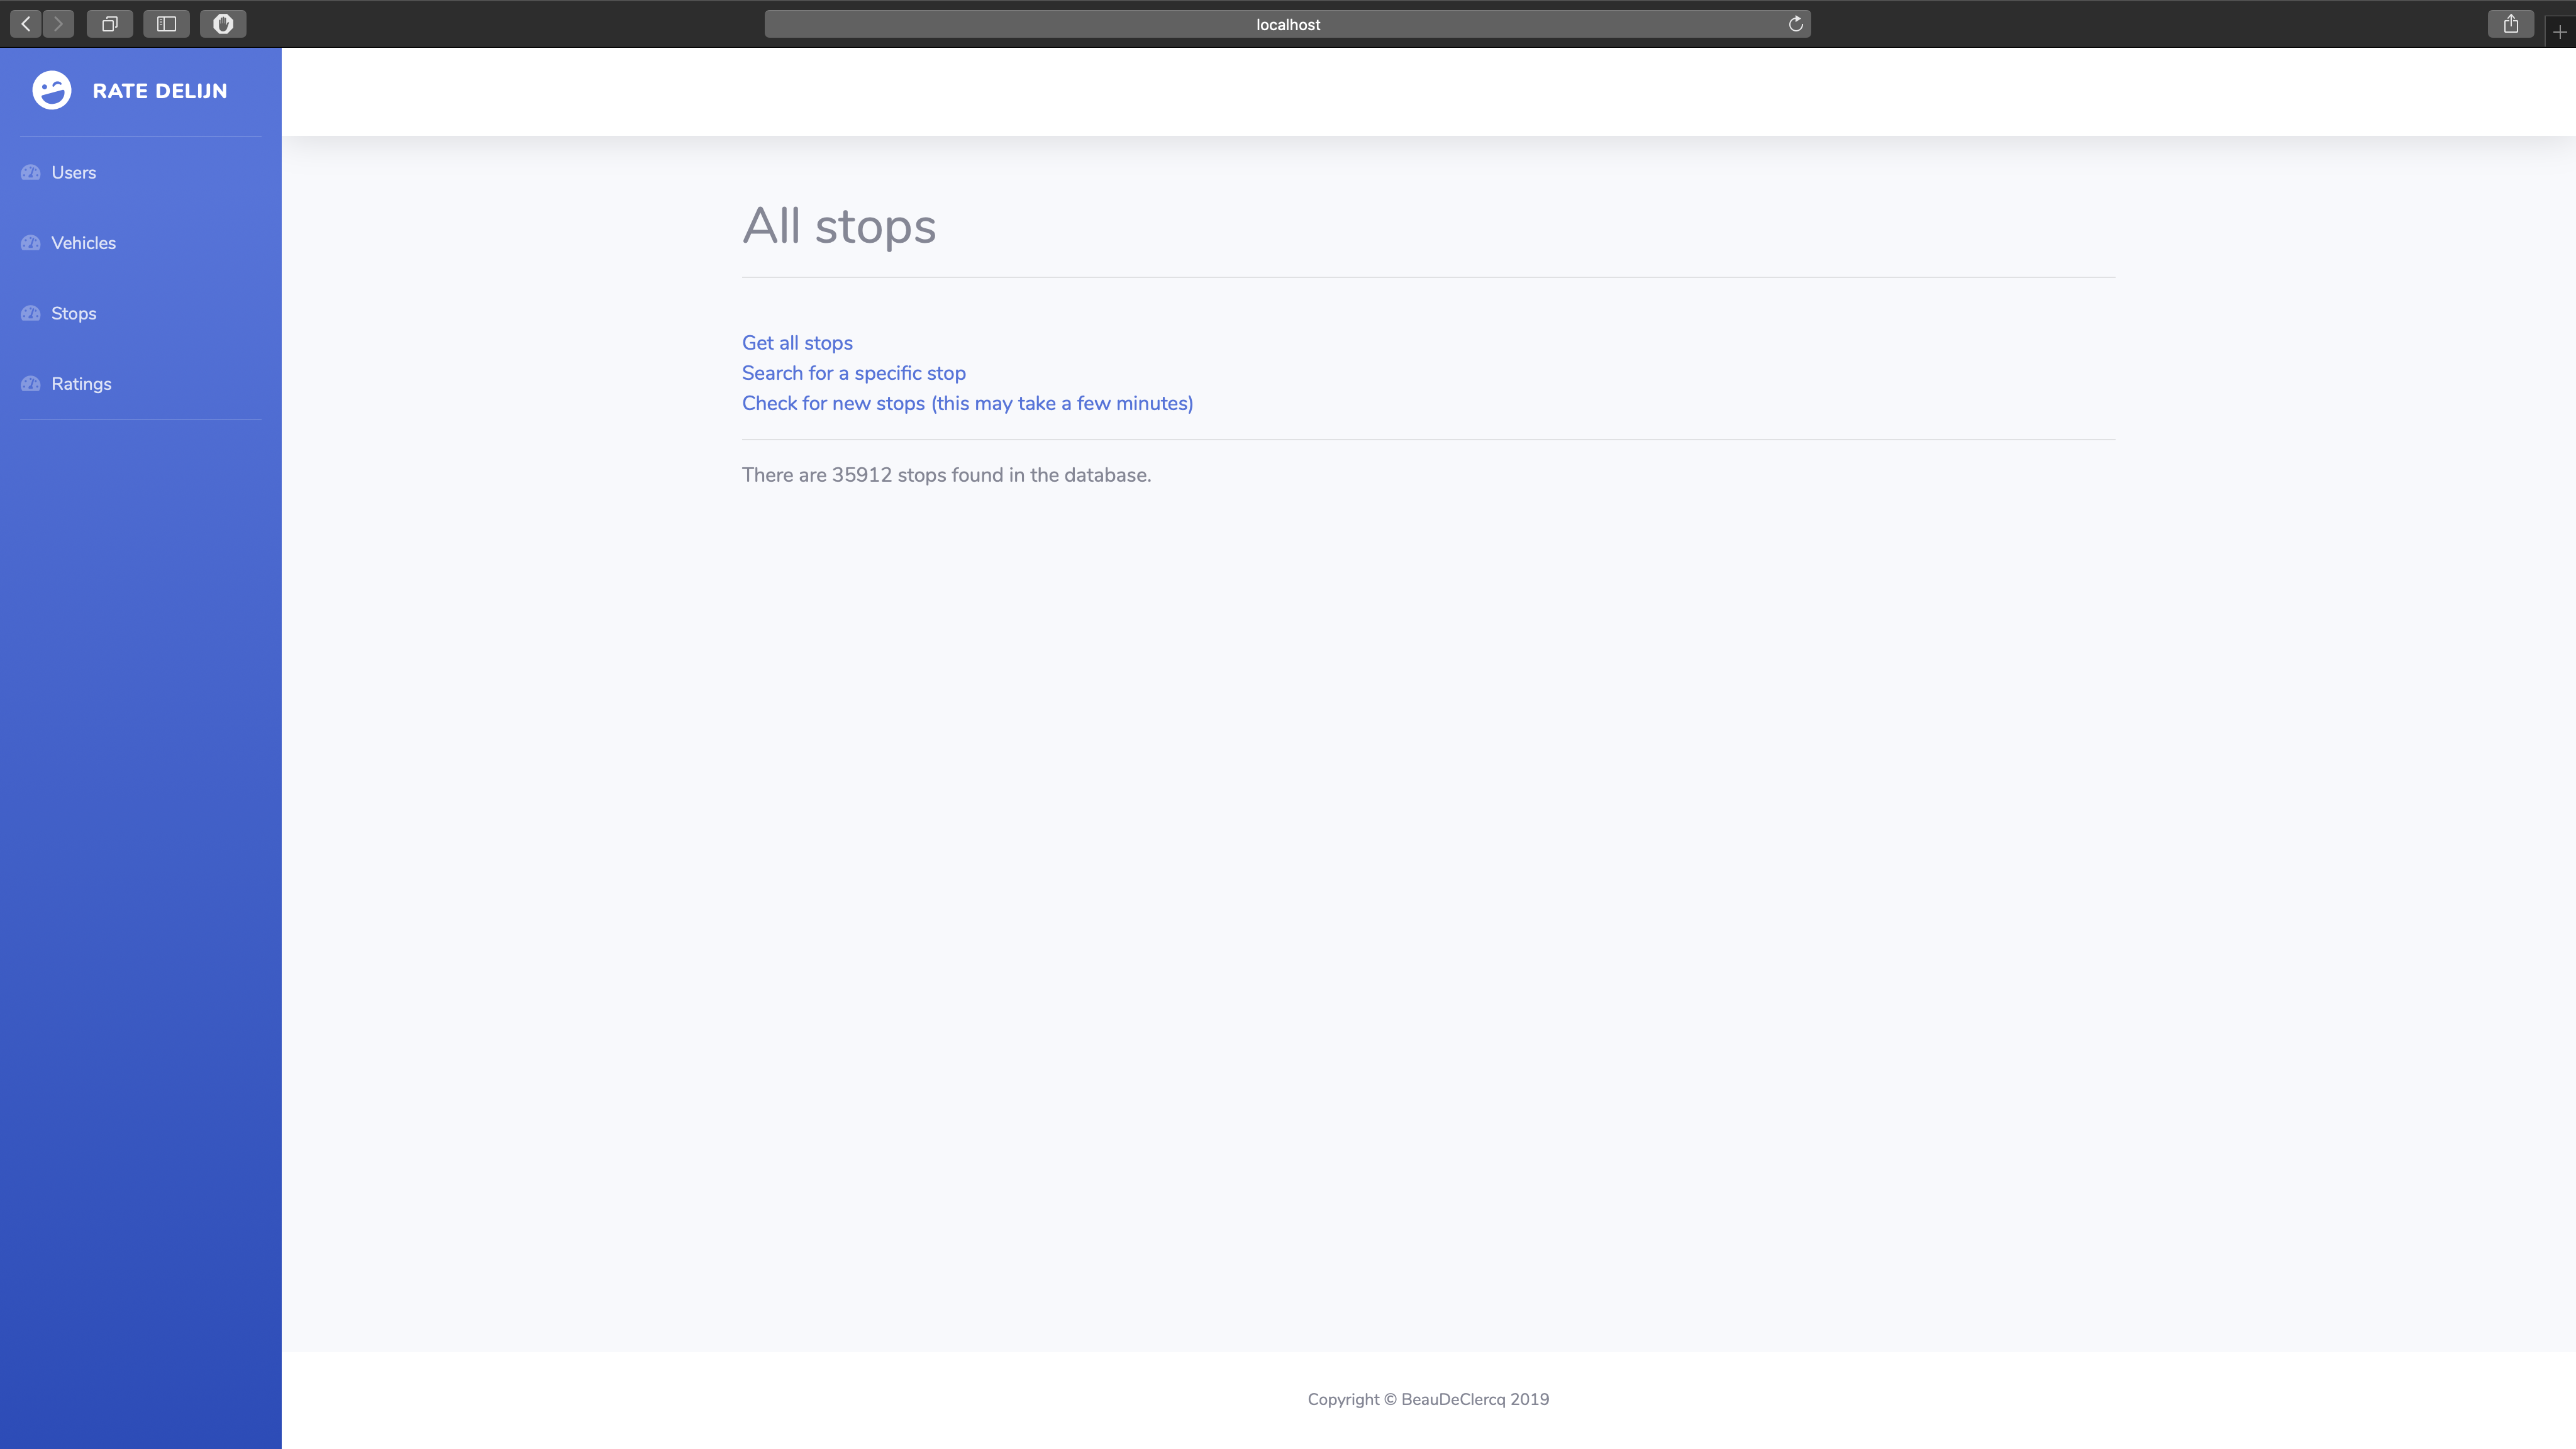
\includegraphics[width=\linewidth]{Images/Stops_tab.png}
	\captionof{figure}{Stops tab}
\end{center}
In  the \textbf{Stops} tab, users can view all stops, search for a specific stop or update the database if they think new stops have been added by DeLijn.

\subsubsection{View all stops}
\begin{center}
	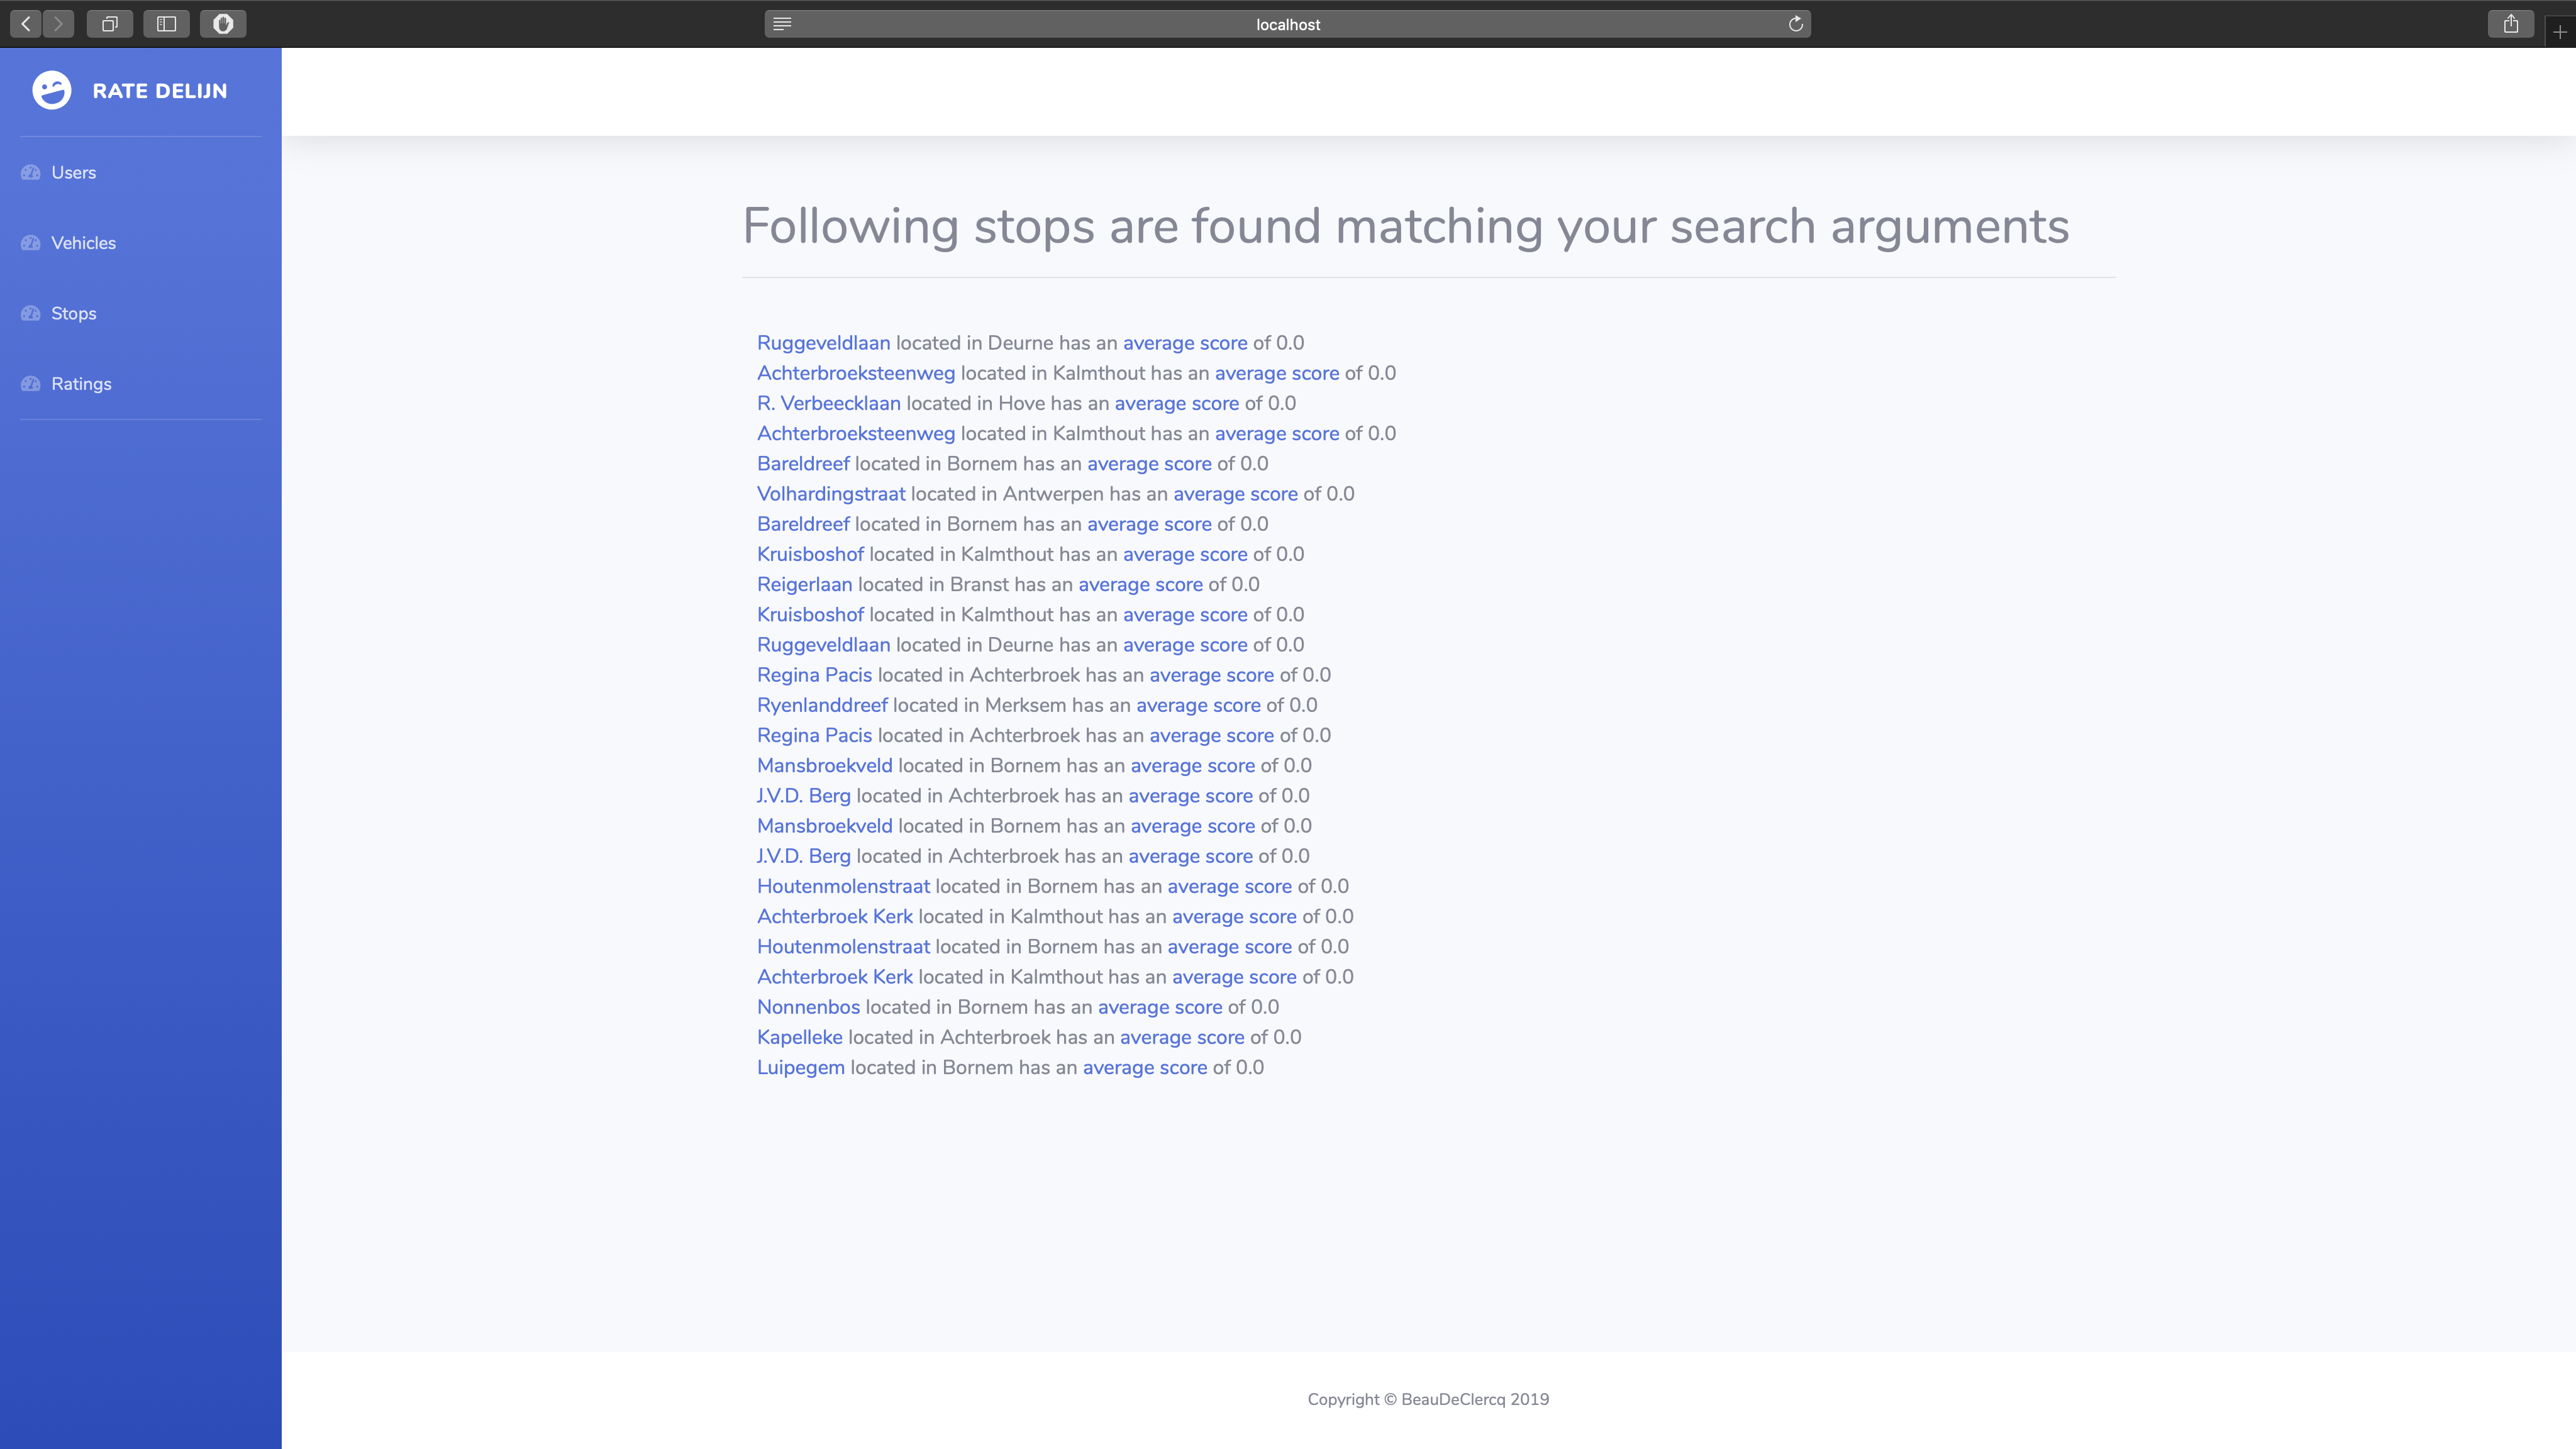
\includegraphics[width=\linewidth]{Images/All_stops.png}
	\captionof{figure}{List of all stops}
\end{center}
On this page, the user will get an unsorted list of all stops currently found in the database.\\
Clicking on the name of the stop will take the user to the rating form for the stop, clicking on the average score will take the user to the detail page for that stop.\\
Using this list is not advised as it may take a minute to load all records.

\subsubsection{Search for a stop}
\begin{center}
	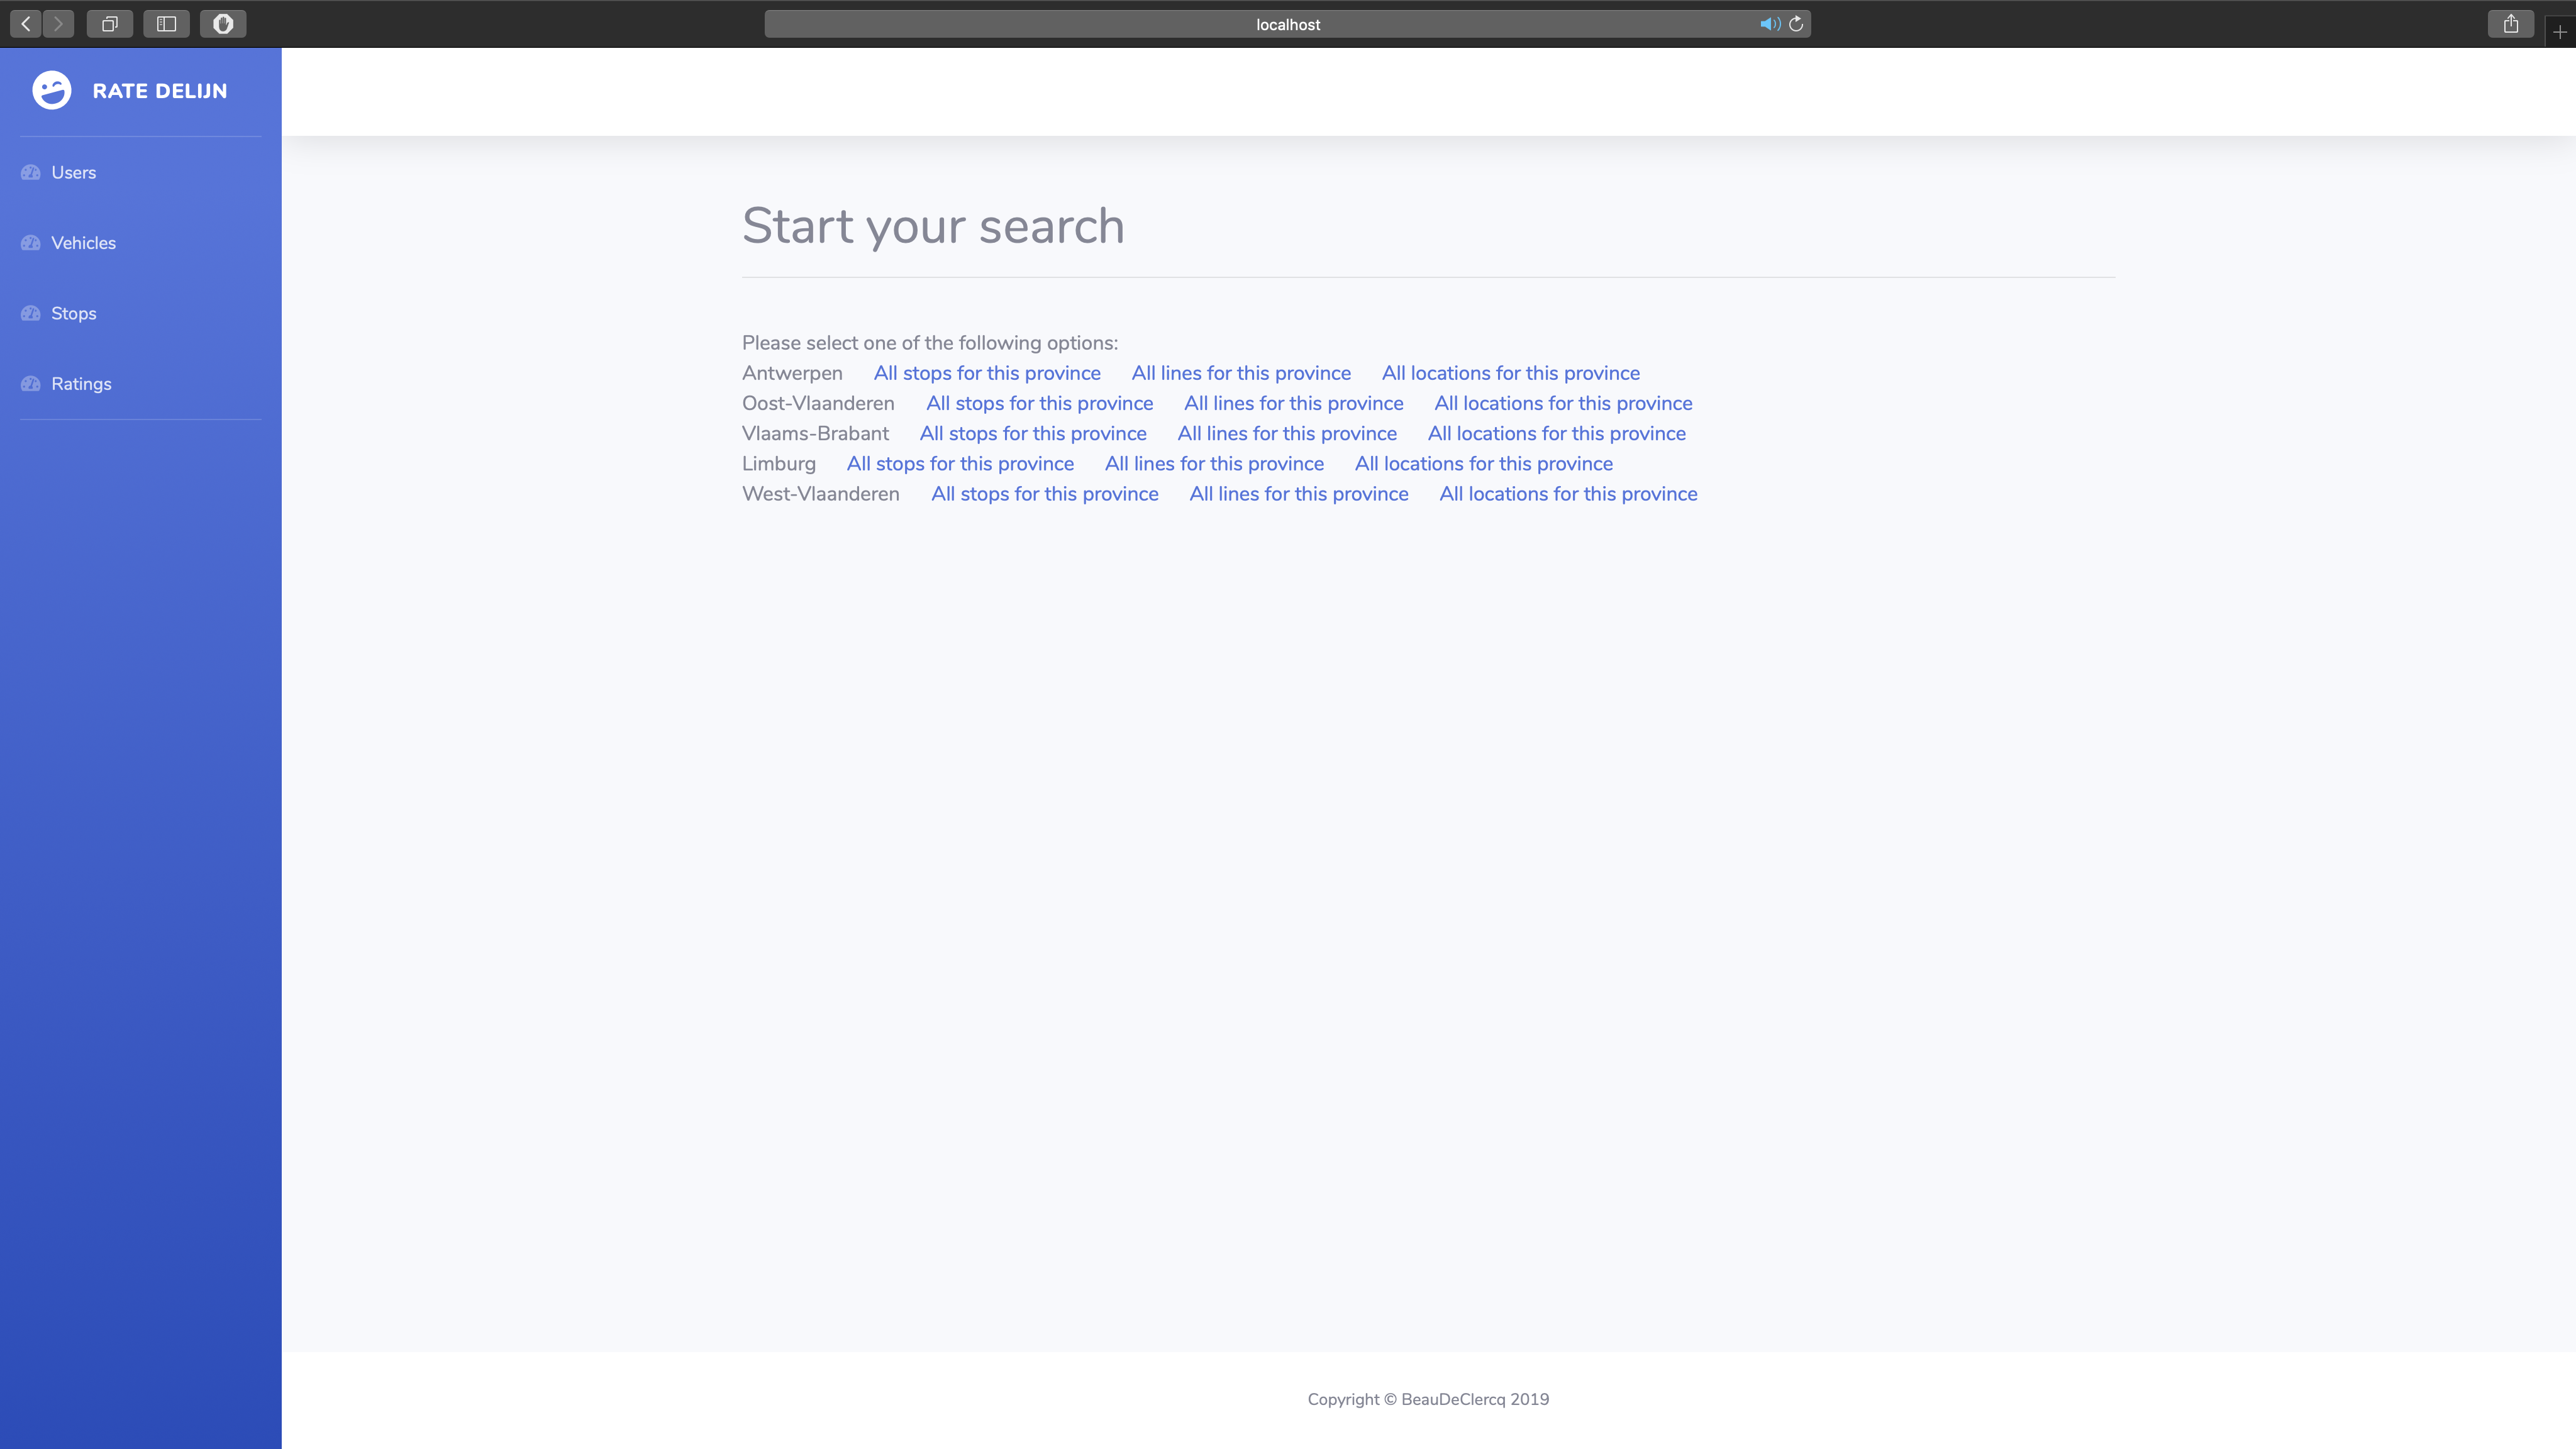
\includegraphics[width=\linewidth]{Images/Start_search.png}
	\captionof{figure}{Start searching for a stop}
\end{center}
There are a few options for a user who want to search for a specific stop:
\begin{itemize}
	\item Per province: if the user wants a list of all stops for a province, this is the desired option.
	\item Per line: if the user wants a list of all stops for a certain line, this is the desired option.
	\item Per town: if the user wants a list of all stops for a certain location, this is the desired option.
\end{itemize}

\subsubsection{Search for a stop: per province}
\begin{center}
	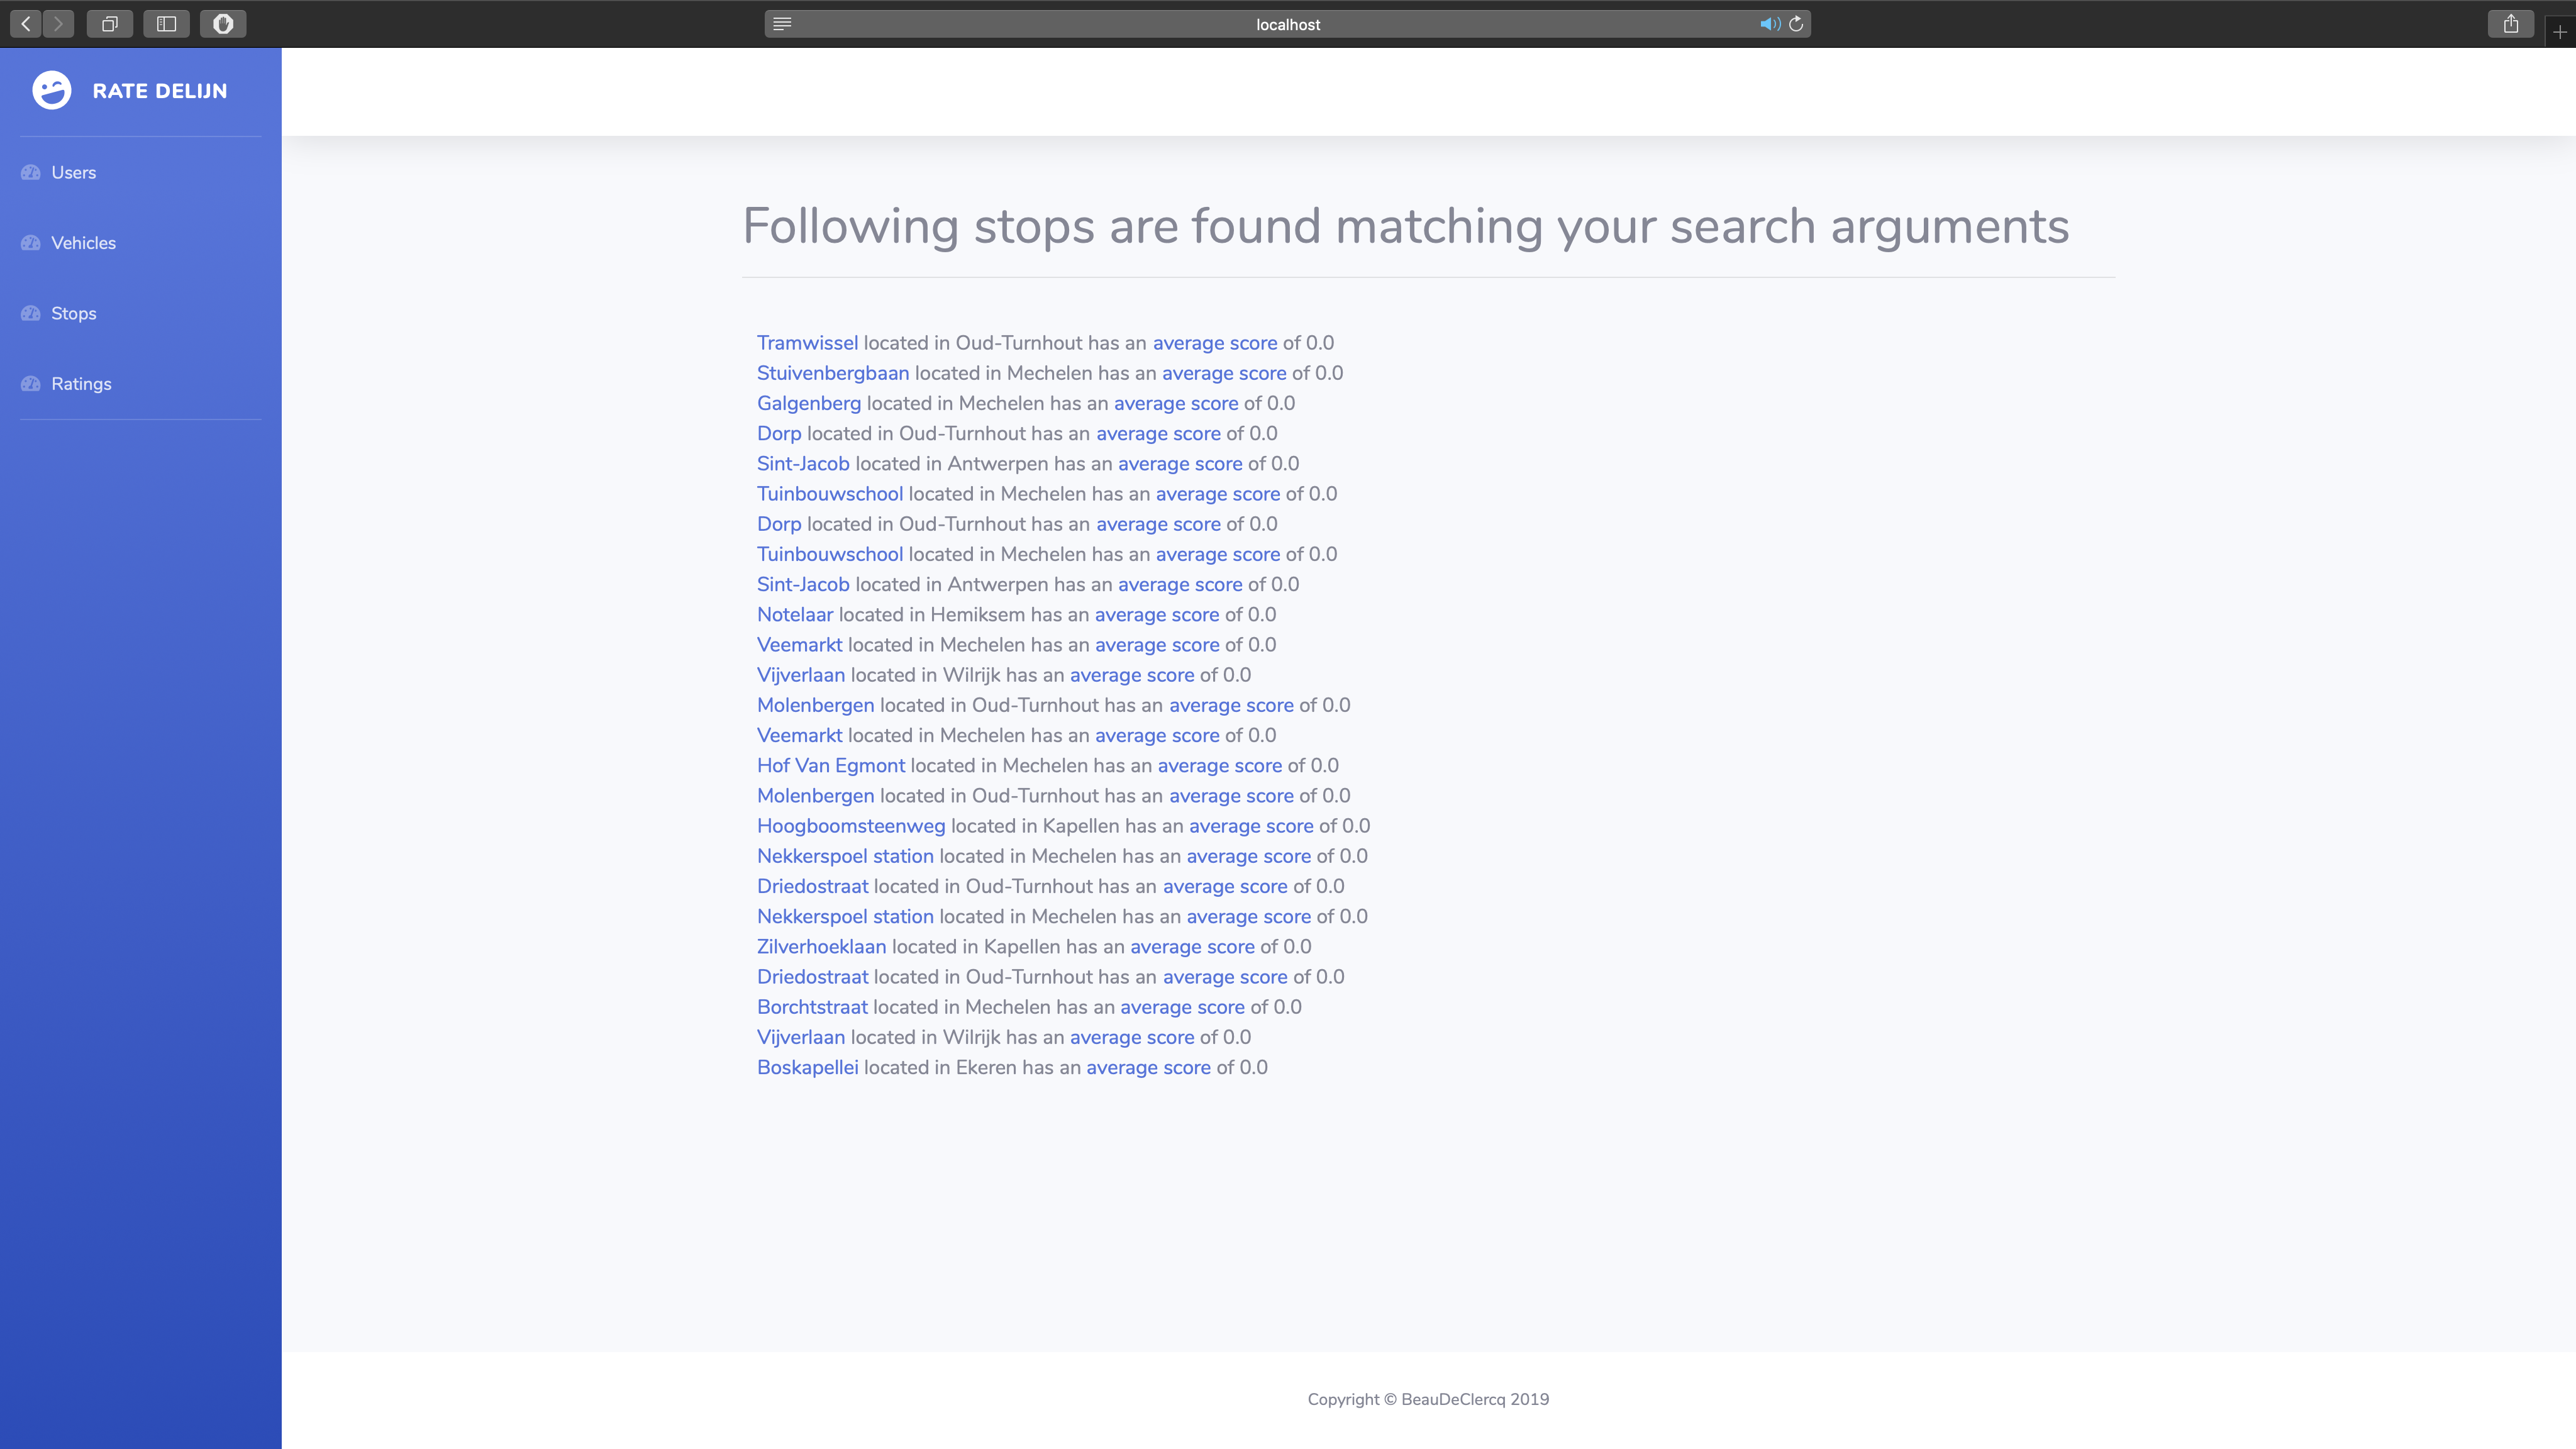
\includegraphics[width=\linewidth]{Images/Stops_province.png}
	\captionof{figure}{Stops per province}
\end{center}
If the option `All stops for this province' was selected, the user will be shown an unordered list of all stops for the chosen province.\\
Clicking on the name of the stop will take the user to the rating form for the stop, clicking on the average score will take the user to the detail page for that stop.\\

\subsubsection{Search for a stop: per line}
\begin{center}
	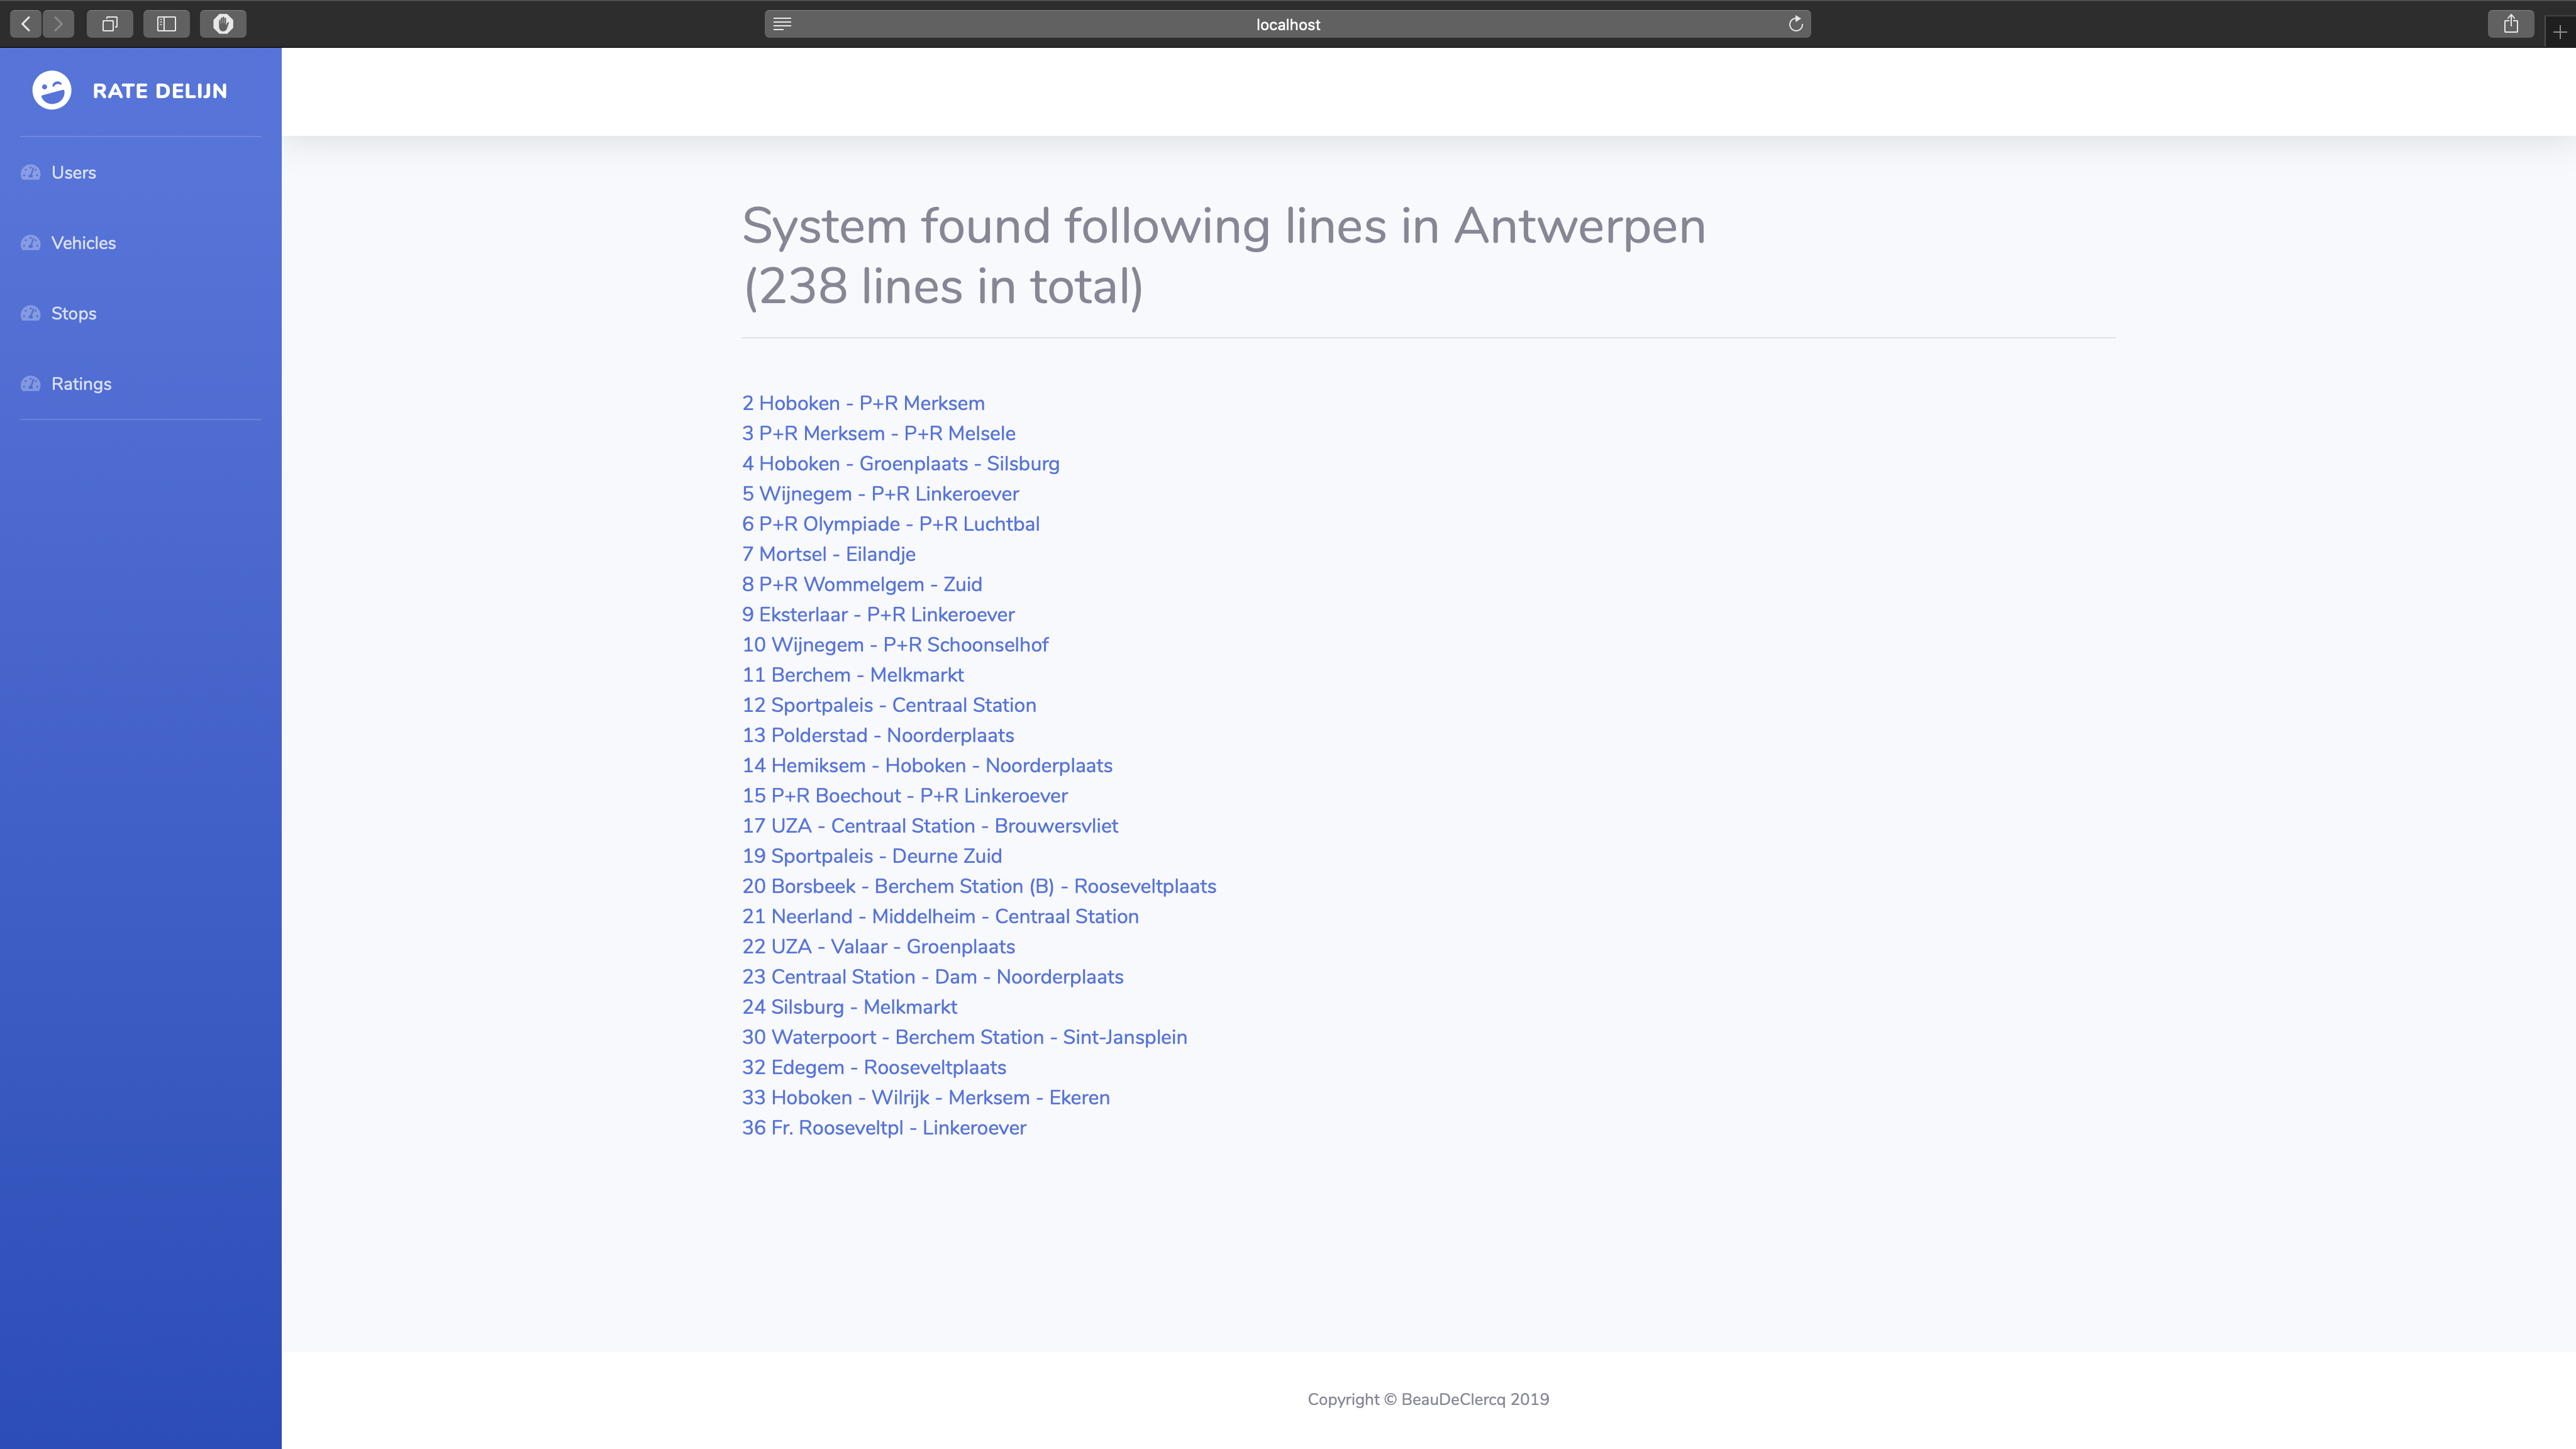
\includegraphics[width=\linewidth]{Images/Lines_province.png}
	\captionof{figure}{Lines per province}
\end{center}
If the option `All lines for this province' was selected, the user will be shown a list of all lines for the chosen province.\\
Selecting one of these lines will give the user a list of all available stops for that line. Clicking on the name of the stop will take the user to the rating form for the stop, clicking on the average score will take the user to the detail page for that stop.\\

\subsubsection{Search for a stop: per town}
\begin{center}
	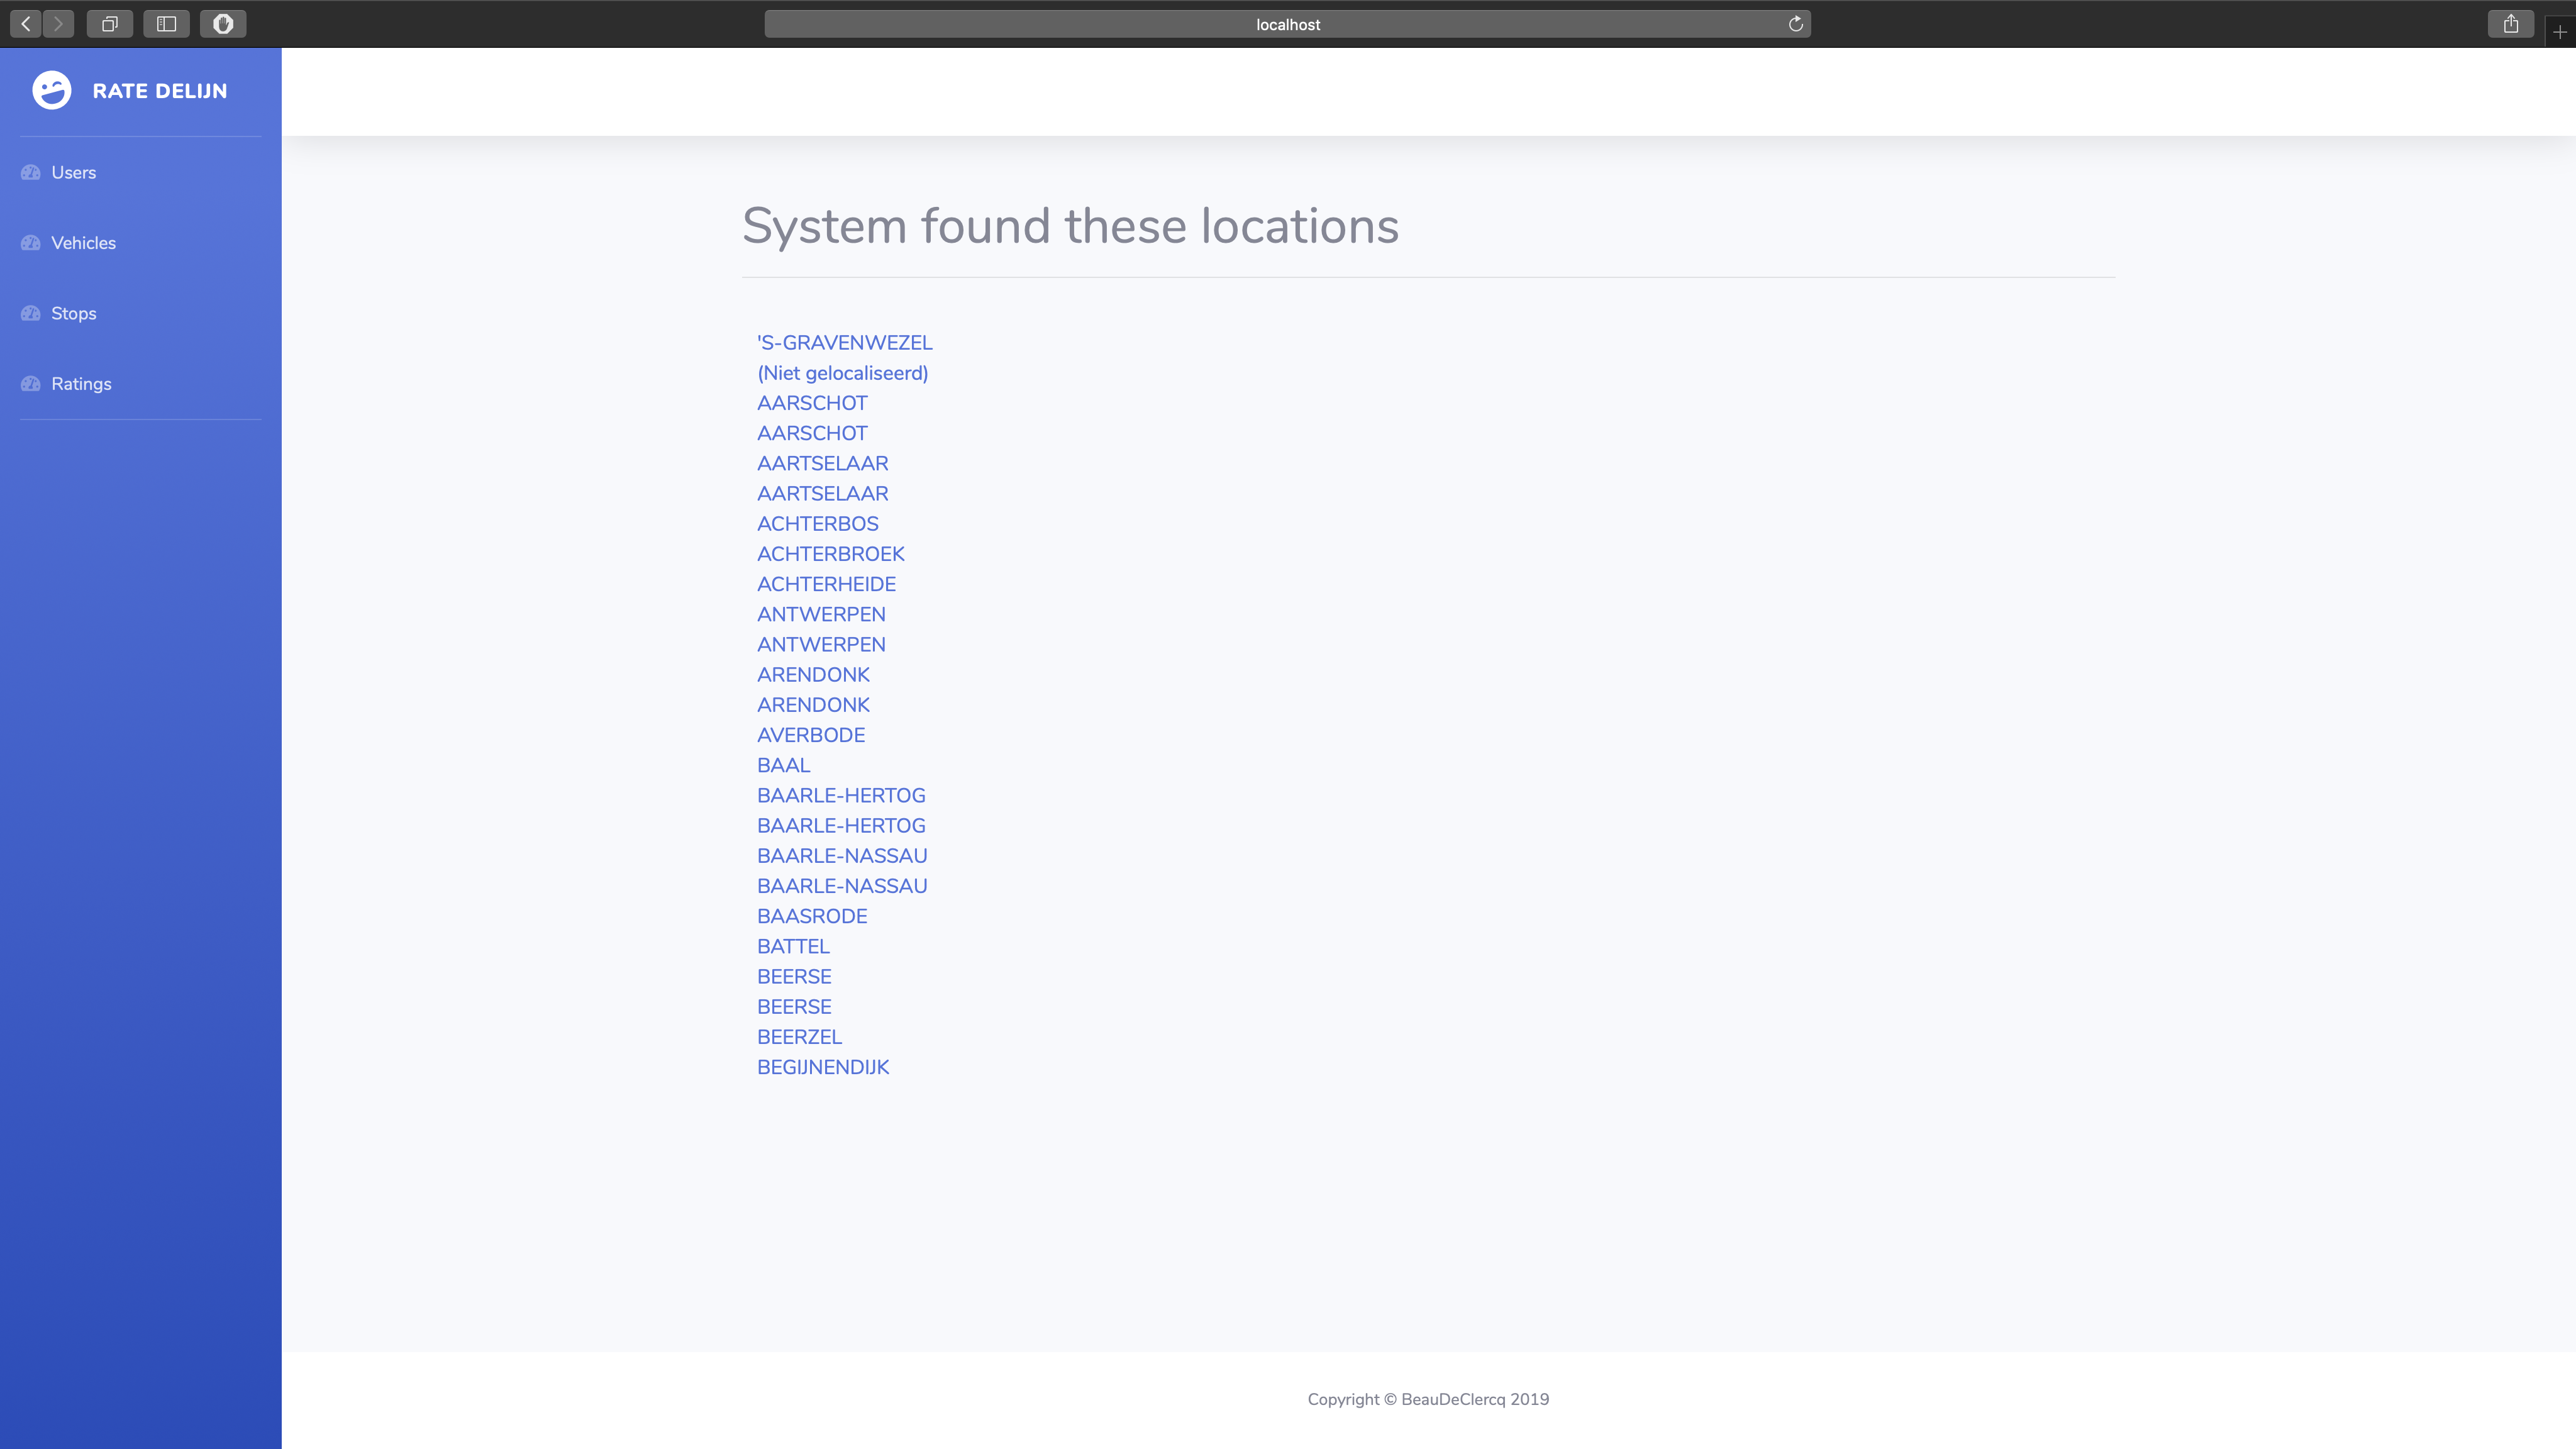
\includegraphics[width=\linewidth]{Images/Locations_province.png}
	\captionof{figure}{Locations per province}
\end{center}
If the option `All locations for this province' was selected, the user will be shown a list of all towns for the chosen province.\\
Selecting one of these locations will give the user a list of all available stops in that location. Clicking on the name of the stop will take the user to the rating form for the stop, clicking on the average score will take the user to the detail page for that stop.\\

\subsubsection{Stop details}
\begin{center}
	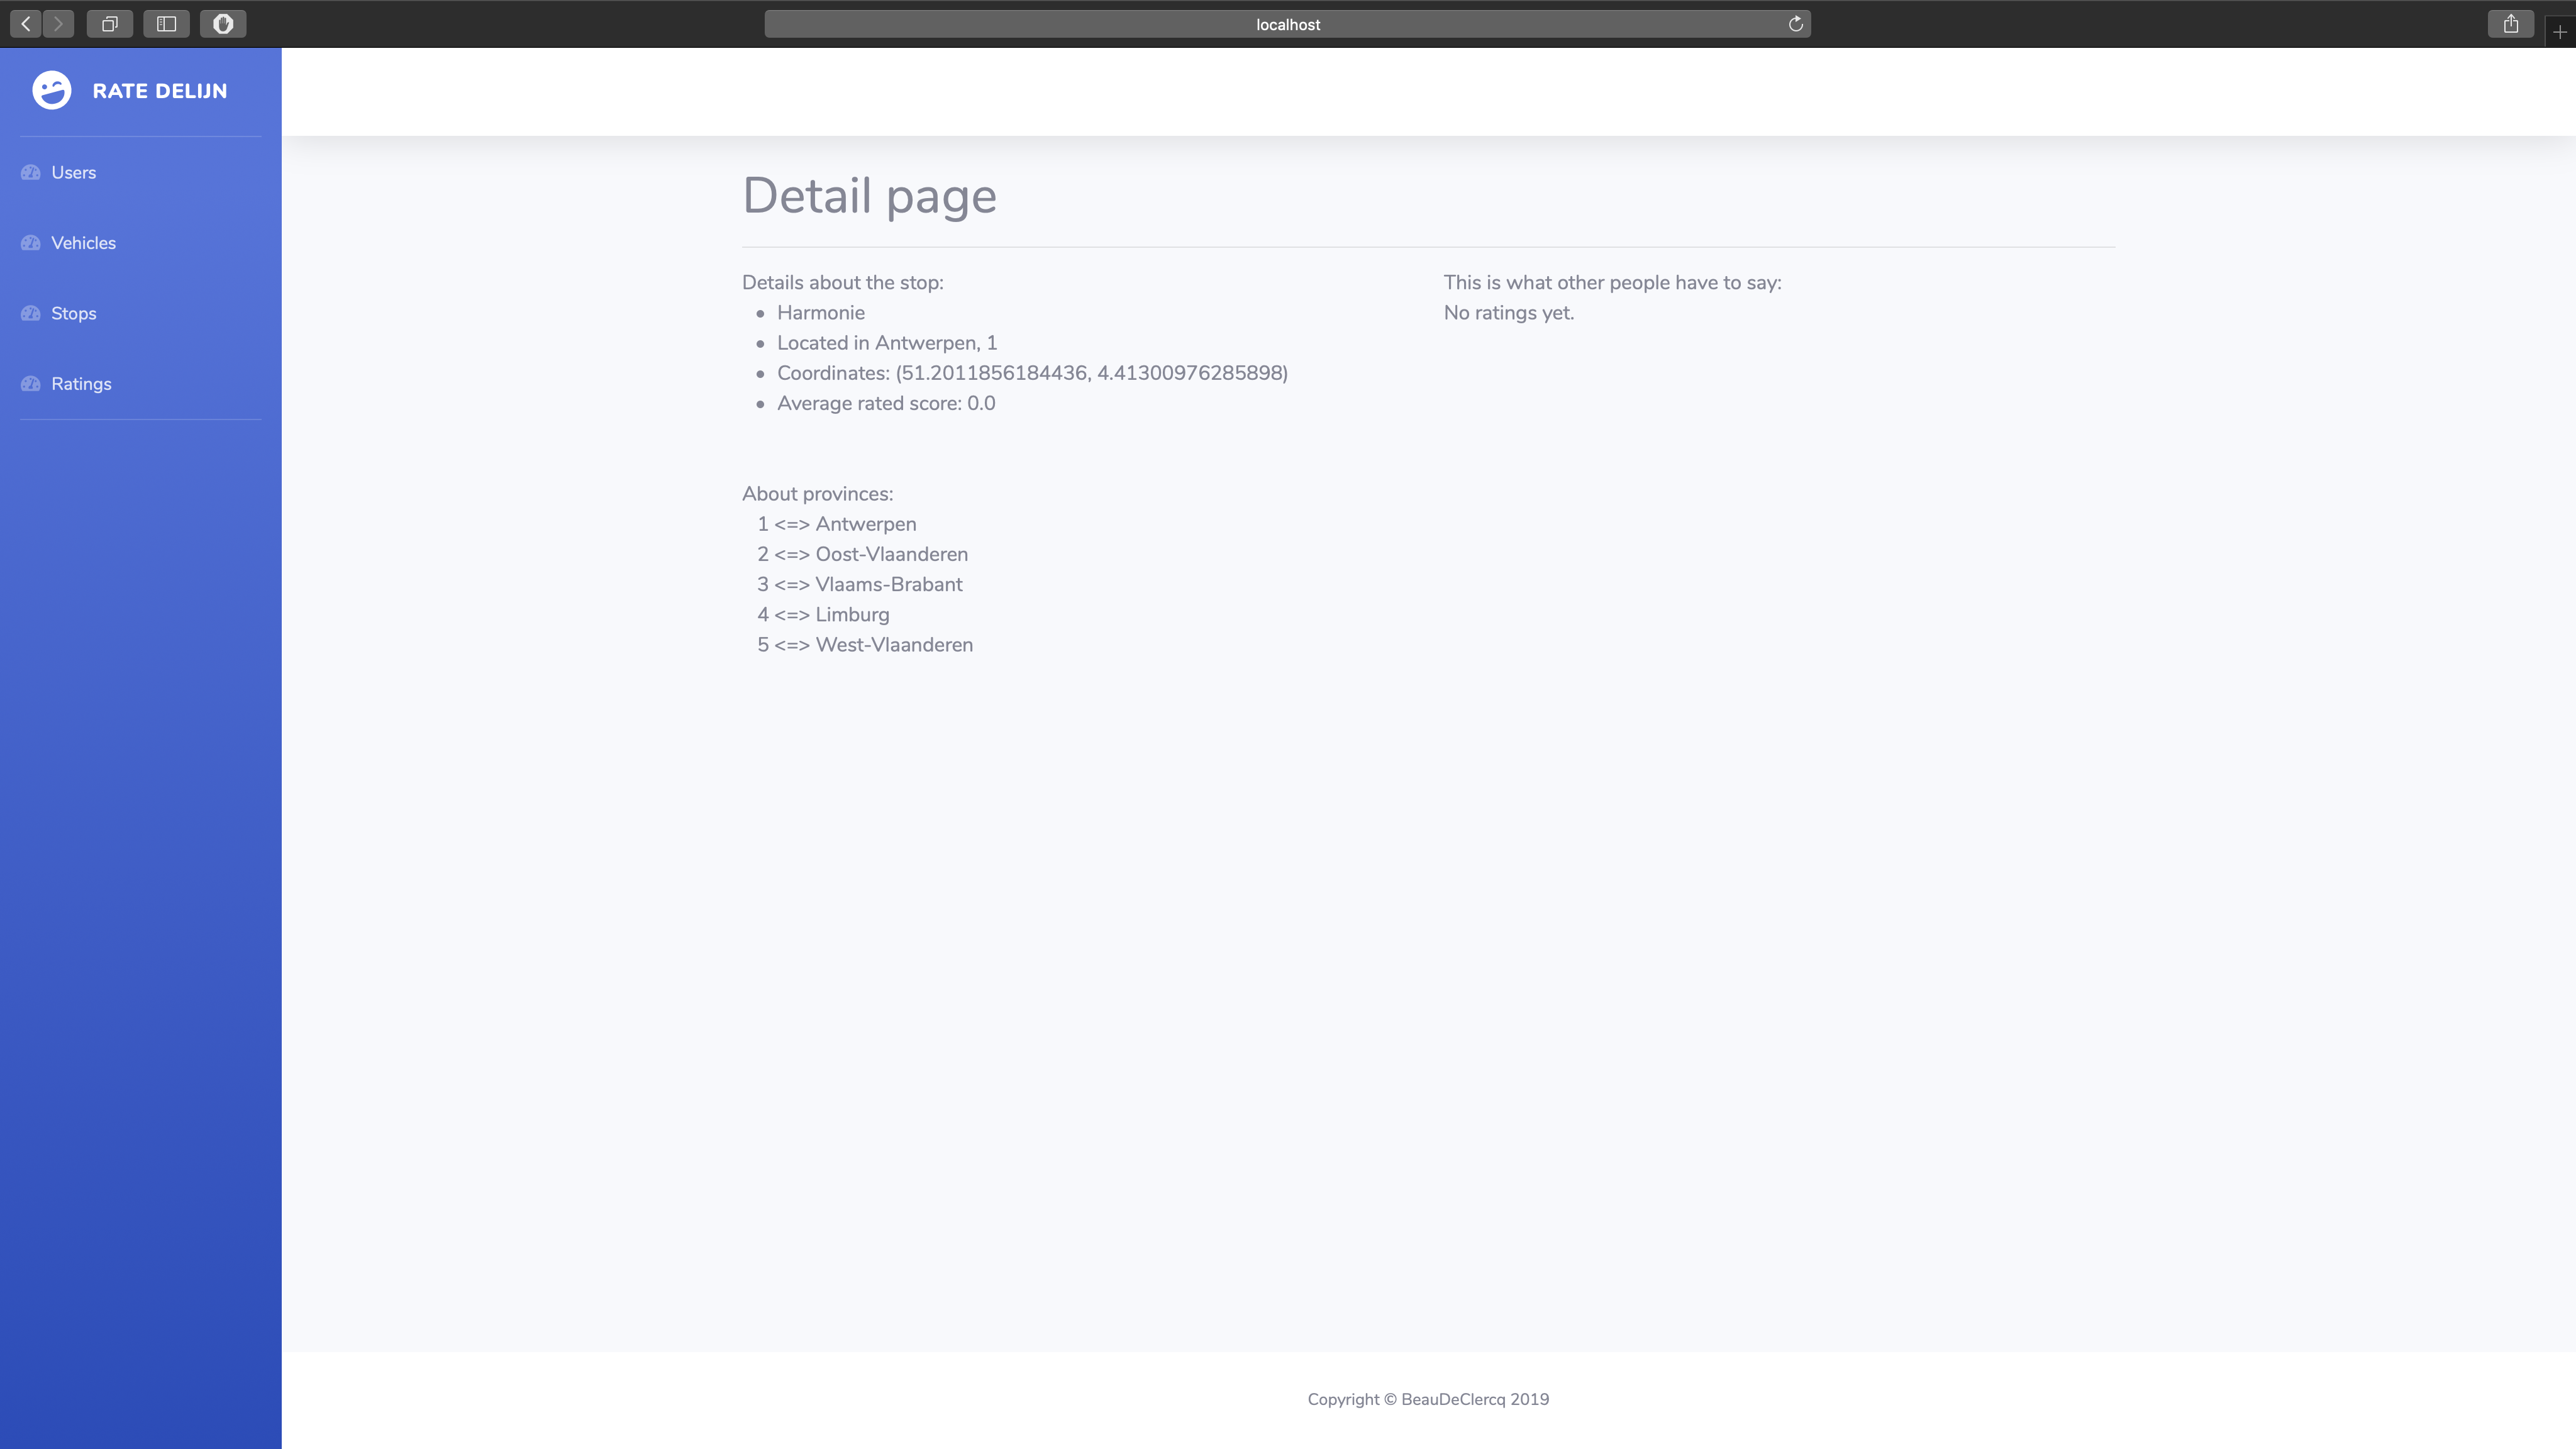
\includegraphics[width=\linewidth]{Images/Stop_details.png}
	\captionof{figure}{Details for a stop}
\end{center}
On the details page, a user can see all details about a stop and read all ratings it has received.

\subsection{Ratings tab}
\begin{center}
	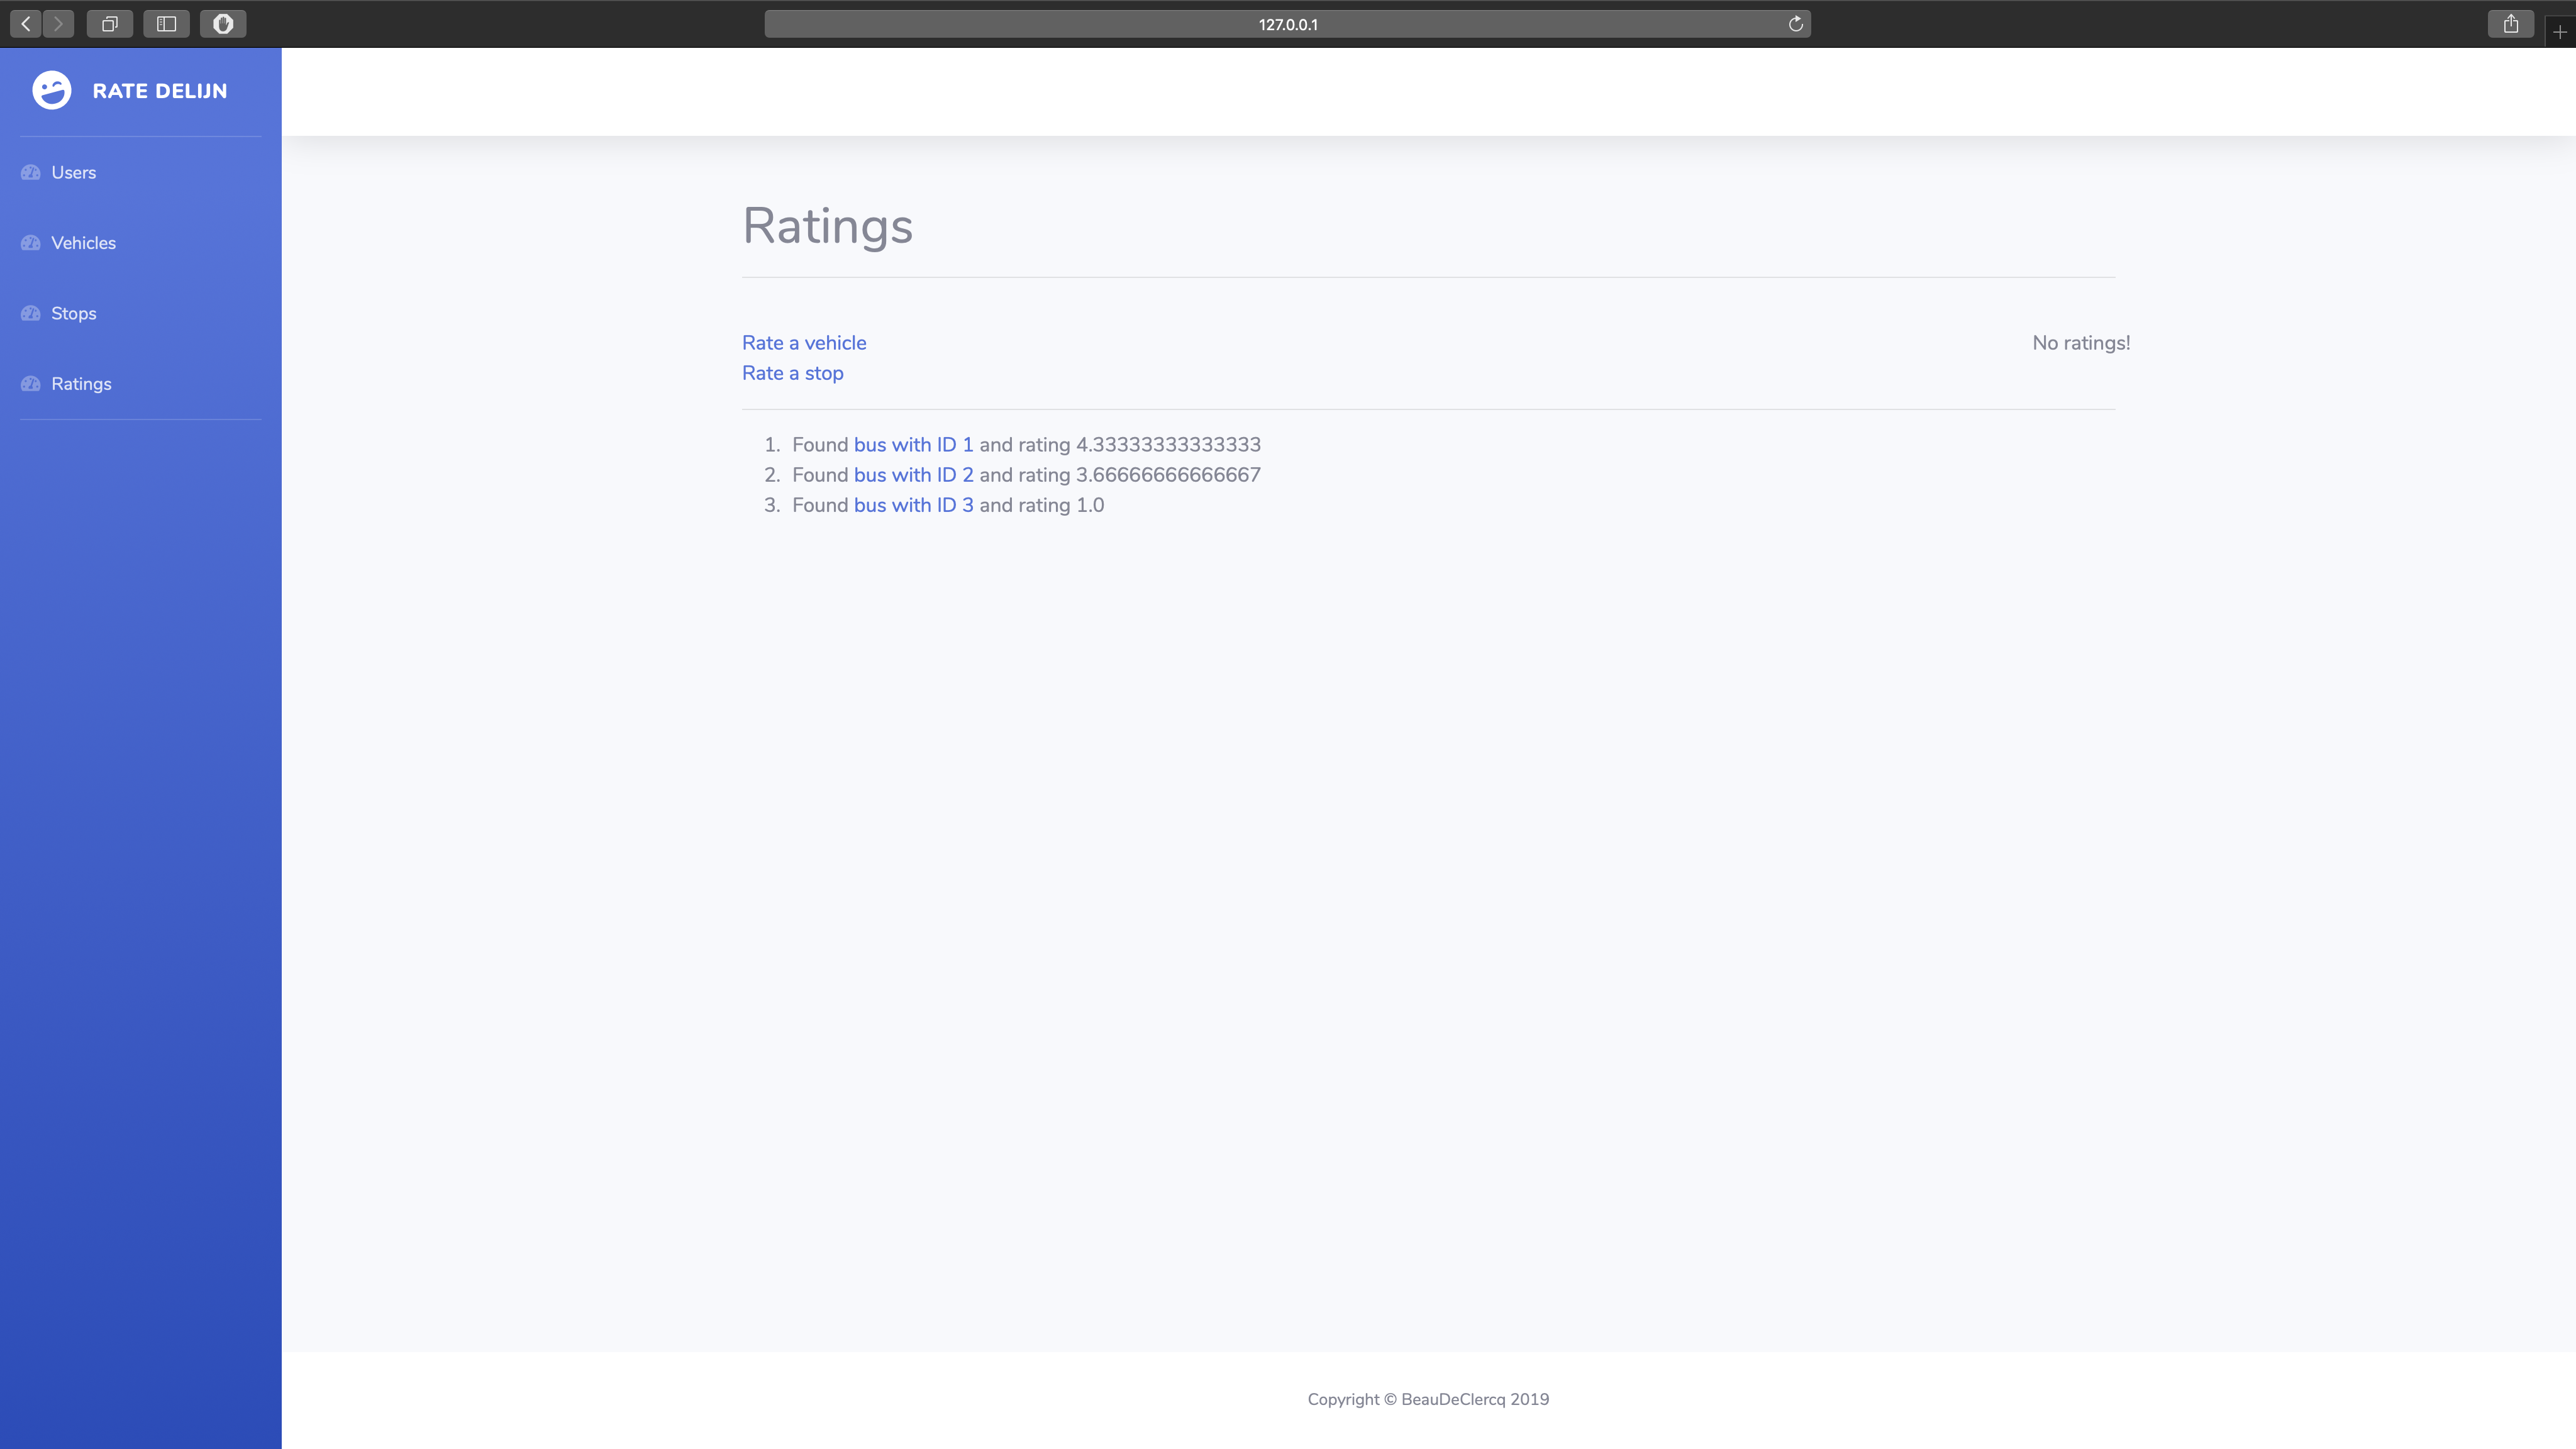
\includegraphics[width=\linewidth]{Images/Ratings_tab.png}
	\captionof{figure}{Ratings tab}
\end{center}
In the \textbf{Ratings} tab, users can choose to rate a vehicle or stop as well as see all ratings currently stored in the database.\\
Clicking on a vehicle from the list will take the user to the details page for that vehicle.

\subsubsection{Rating a vehicle}
\begin{center}
	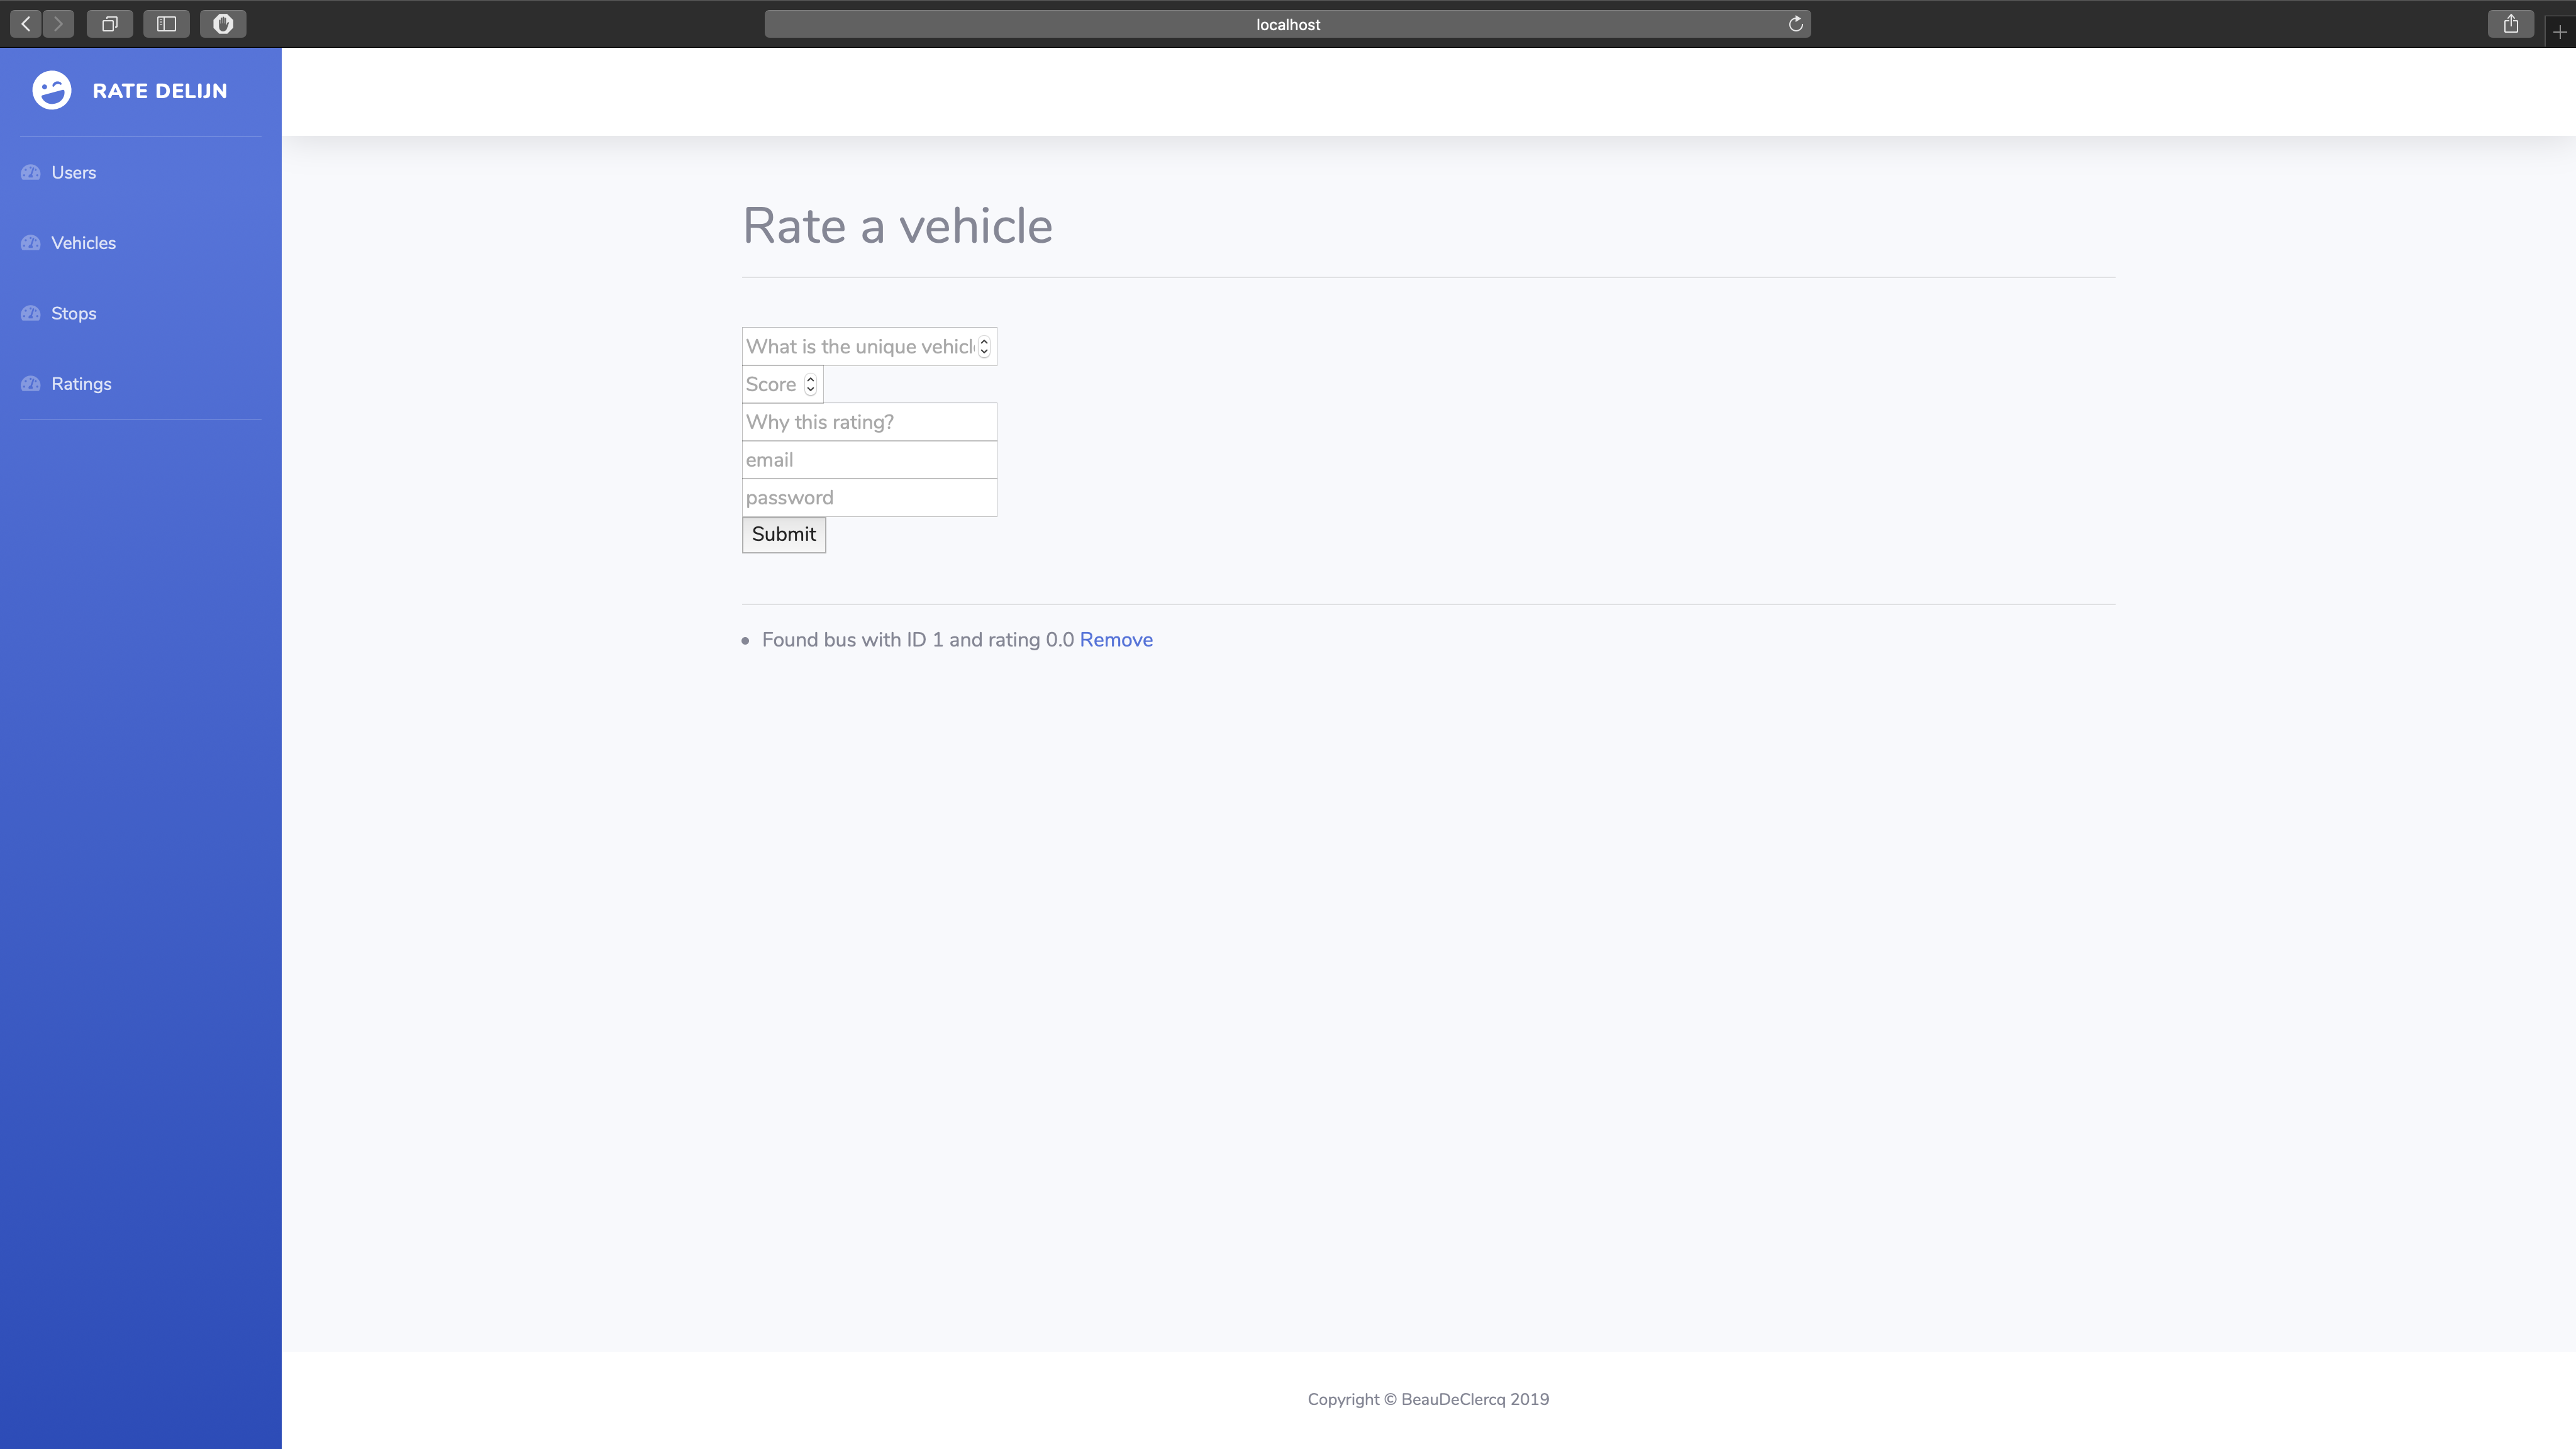
\includegraphics[width=\linewidth]{Images/Rate_vehicle.png}
	\captionof{figure}{Rating a vehicle}
\end{center}
A vehicle can be rated by filling in the form and authenticating. \\
Once the form is submitted, the user will be redirected to the home page where a message will be shown telling whether the operation was successful or not.

\subsubsection{Rating a stop}
\begin{center}
	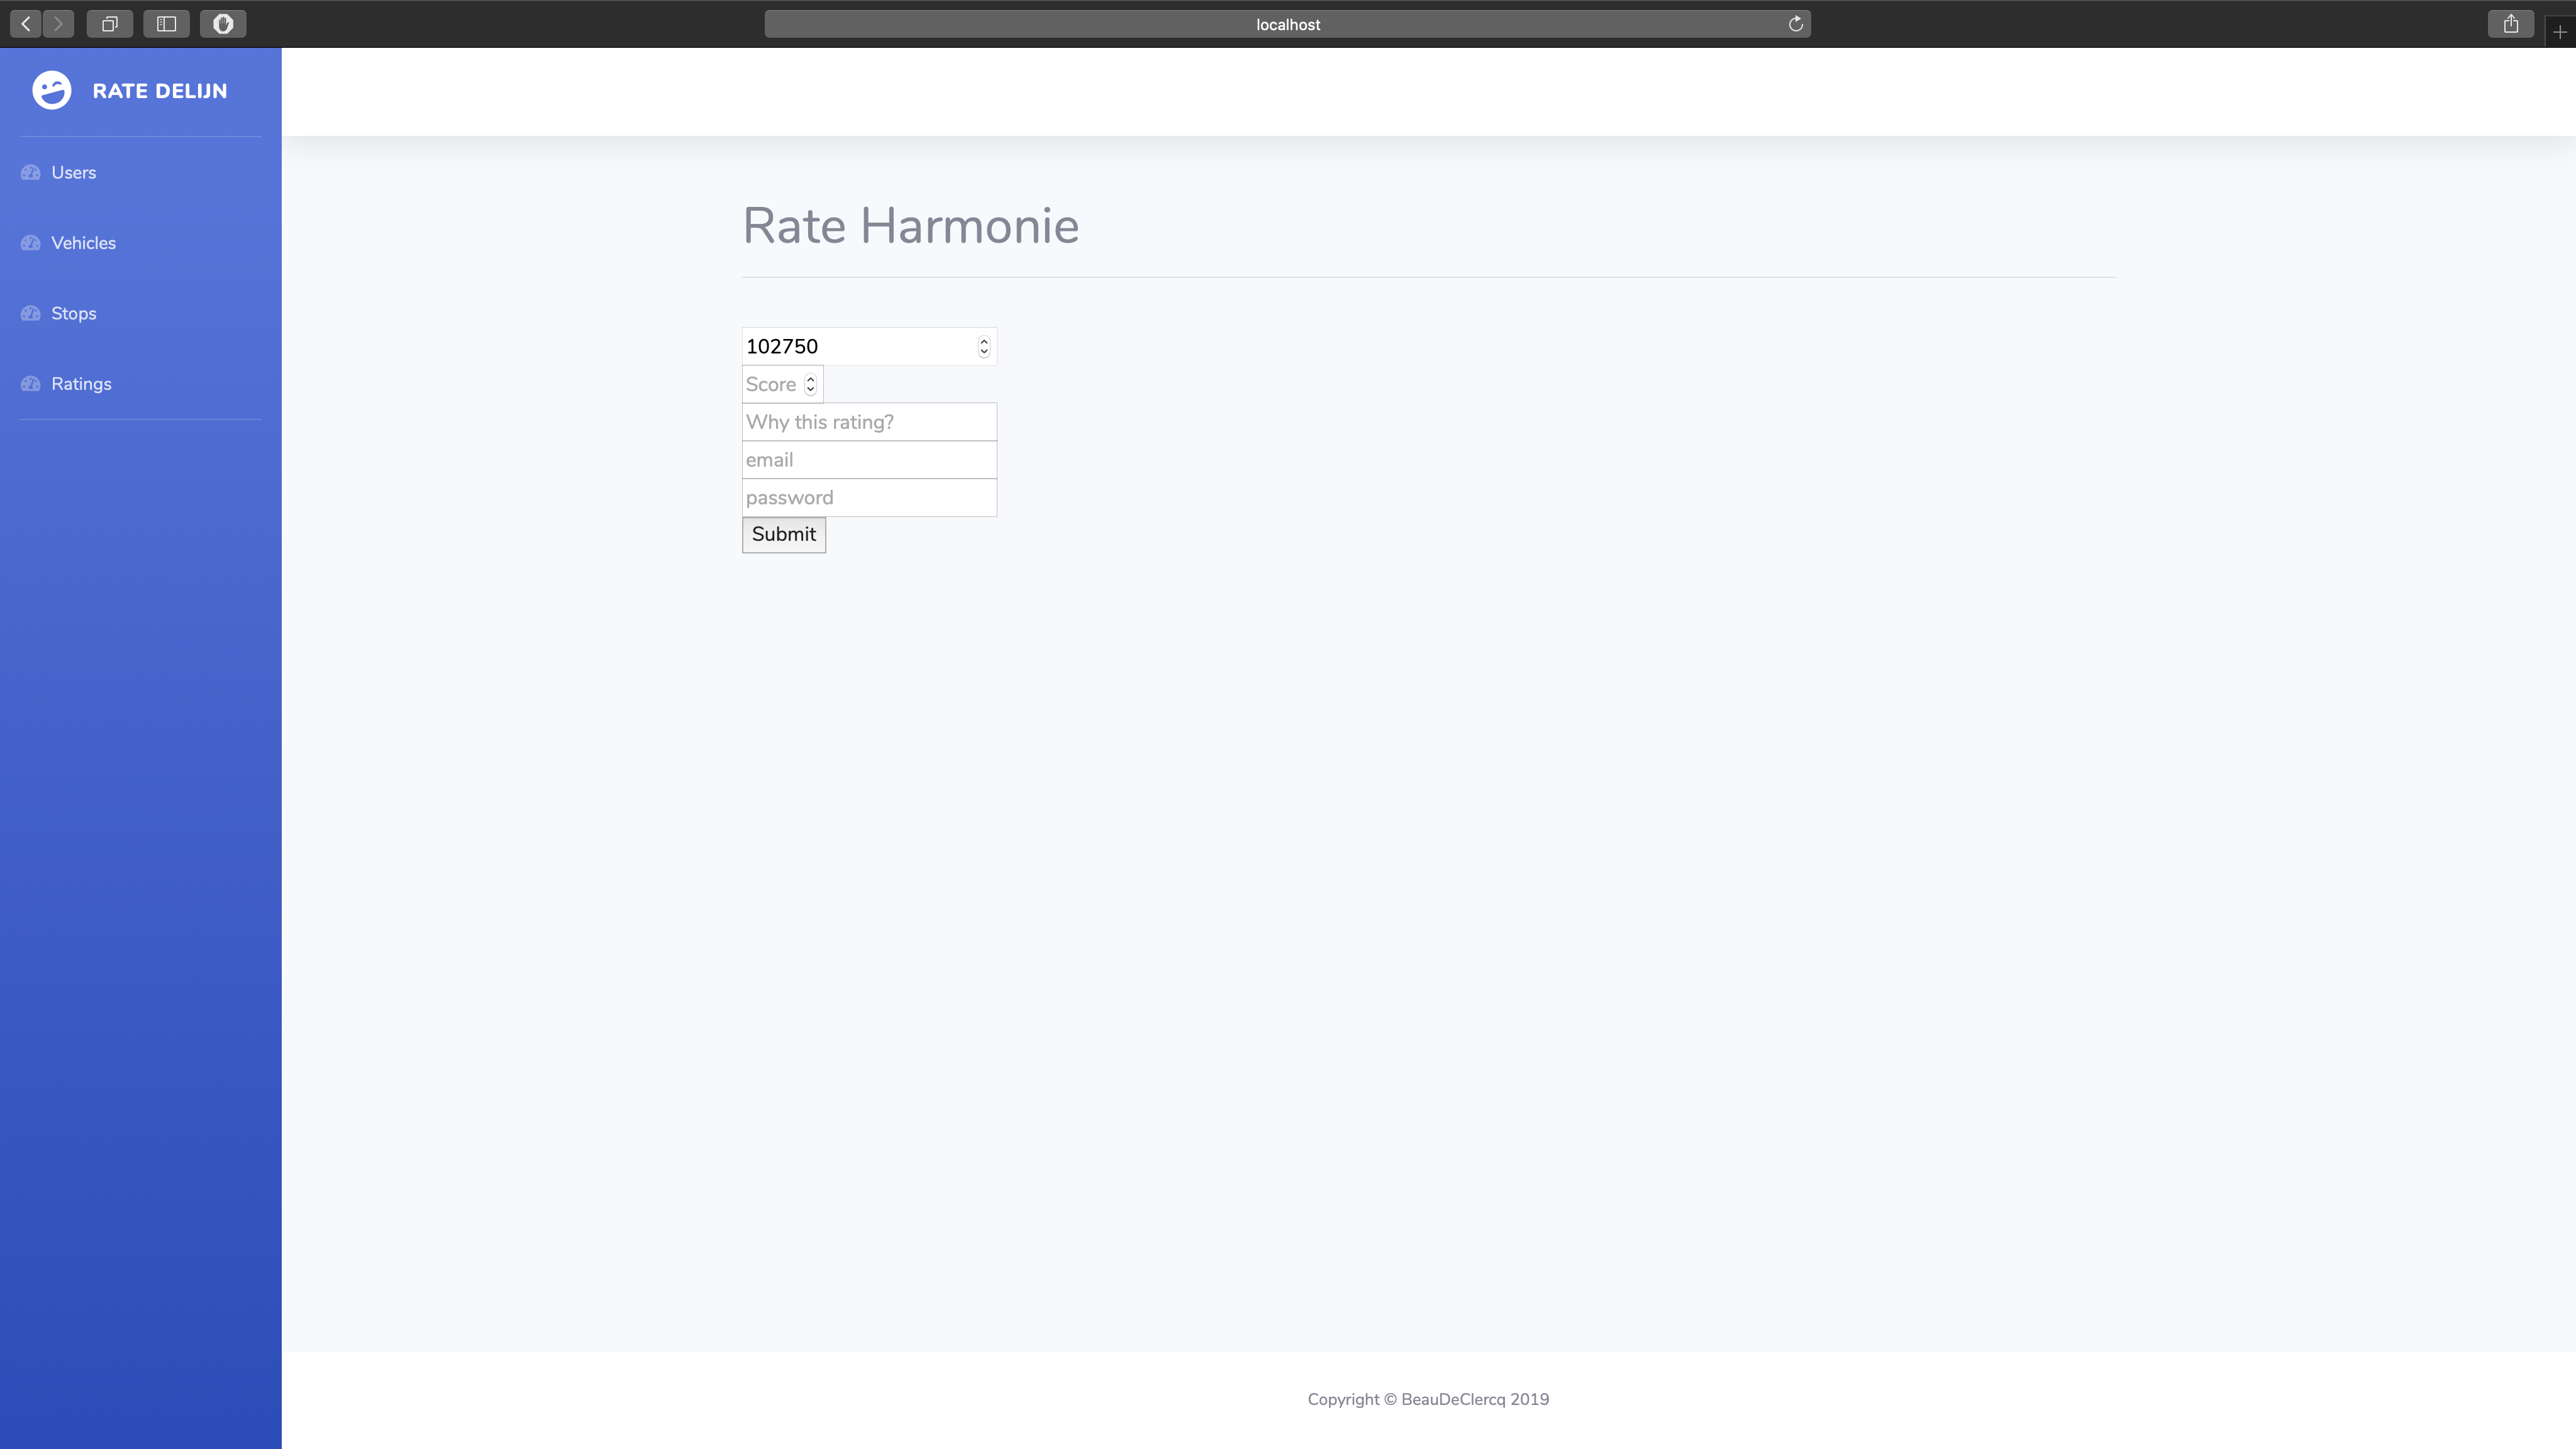
\includegraphics[width=\linewidth]{Images/Rate_stop.png}
	\captionof{figure}{Rating a stop}
\end{center}
Selecting the `Rate a stop' option will take the user to the search page for a stop. When the desired stop is found, the user simply needs to click on the name of the stop to be redirected to the rating form.\\
Once the form is submitted, the user will be redirected to the home page where a message will be shown telling whether the operation was successful or not.

\subsubsection{Updating a review}
If a user would like to update their review, all they need to do is fill out the form again and submit it.

\subsubsection{Removing a review}
If a user would like to remove their review, they can do so by going to the corresponding stop or vehicle details page. There the user can select the `Remove your rating' option.
\newpage

\section{Architecture}
The application consists of 5 services: \textbf{Users}, \textbf{Vehicles}, \textbf{Stops}, \textbf{Ratings} and \textbf{Interface}.\\
The \textbf{Users}, \textbf{Vehicles}, \textbf{Stops} and \textbf{Ratings} service each have their own database. 

\subsection{Users service}
The \textbf{Users} service handles all things related to registering and authenticating users. This service makes no calls to any other services.\\ 
Email-password combinations are stored in the database belonging to this service.

\subsection{Vehicles service}
The \textbf{Vehicles} service handles all things related to adding and removing a vehicle, updating the average score and retrieving a certain vehicle. This service makes calls to the \textbf{Users} and \textbf{Ratings} services.\\
All vehicles are stored in the database belonging to this service.

\subsection{Stops service}
The \textbf{Stops} service handles the searching for a stop and checking for new stops. This service only makes calls to the API of DeLijn and to no other services.\\ 
All stops are stored in the database belonging to this service.

\subsection{Ratings service}
The \textbf{Ratings} service handles the rating of vehicles and stops. This service makes calls to the \textbf{Vehicles}, \textbf{Users} and \textbf{Stops} services.\\
All ratings are stored in the database belonging to this service.

\subsection{Interface service}
The \textbf{Interface} only provides the web pages. This service has no underlying database and makes calls to all other services.

\subsection{Diagram}
\begin{center}
	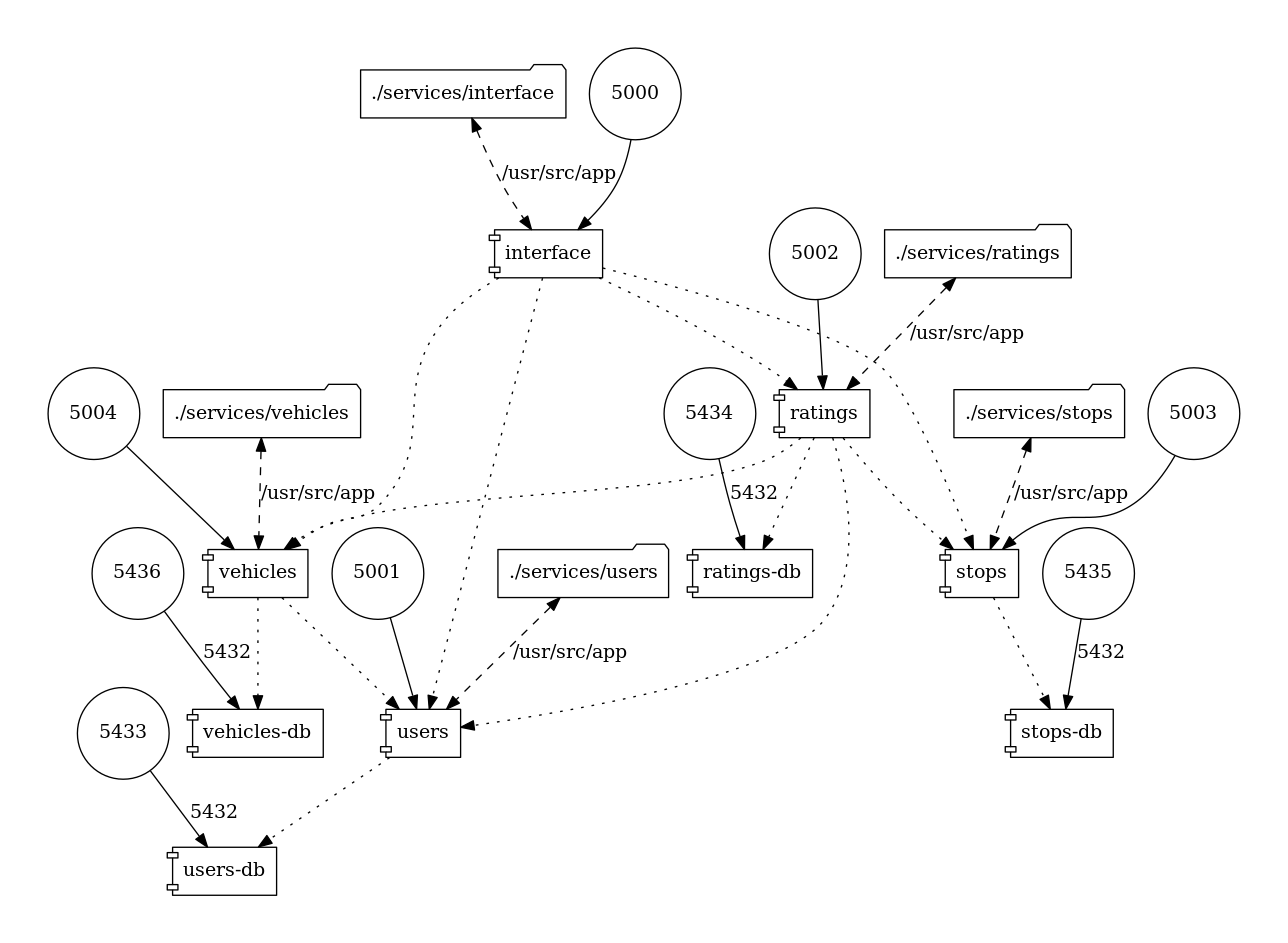
\includegraphics[width=\linewidth]{Images/Architecture.png}
	\captionof{figure}{Architecture}
\end{center}
This diagram was automatically generated based on the \textbf{docker-compose.yml} file by running following command in the root directory:\\
\texttt{docker run --rm -it --name dcv -v \$(pwd):/input pmsipilot/docker-compose-viz render} .

\newpage

\section{Tools and choices}

\subsection{Tools used}
Following tools were used in creating this app:
\begin{itemize}
	\item Basics:
	\begin{itemize}
		\item Flask: framework of the app.
		\item Flask-SQLAlchemy: together with postgresql, this provides the database system of the app.
		\item psycopg2: Python-PostgreSQL Database Adapter.
	\end{itemize}
	\item Others:
	\begin{itemize}
		\item requests module: makes it easier to perform http calls.
	\end{itemize}
\end{itemize}

\subsection{Choices made}
For this project I chose to split the system up in 5 different services because, in my opinion, this best resembled the philosophy of micro-services. Each service can be substituted by another one that provides equal responses to API calls. \\
Since each service has it's own database, no problems regarding data will arise when choosing to swap services.

%\maketitle{Setup}

\end{document}
